\documentclass[sigconf,review, anonymous]{acmart}

\usepackage{booktabs} % For formal tables
\usepackage[utf8]{inputenc}
\usepackage[english]{babel}
\usepackage[T1]{fontenc}
\usepackage{graphicx}
\usepackage{graphics}
\usepackage{listings}  
\usepackage{array}
\newcolumntype{L}[1]{>{\raggedright\let\newline\\\arraybackslash\hspace{0pt}}m{#1}}
\newcolumntype{C}[1]{>{\centering\let\newline\\\arraybackslash\hspace{0pt}}m{#1}}
\newcolumntype{R}[1]{>{\raggedleft\let\newline\\\arraybackslash\hspace{0pt}}m{#1}}
\usepackage{multirow}
%\usepackage[table]{xcolor}
\usepackage{float}
\usepackage{array}
\usepackage{ragged2e}
\usepackage{cleveref}
\usepackage{subcaption}
\usepackage{tikz}
\usepackage[normalem]{ulem}

\newcolumntype{P}[1]{>{\RaggedRight\hspace{0pt}}p{#1}}

\lstset{language=Java,
  tabsize=2,
  basicstyle=\ttfamily\footnotesize,
  moredelim=[is][\dotuline]{@}{@},
  mathescape=true
} 

\newcommand{\squeezeup}{\vspace{-0.5mm}}

\usepackage{etoolbox}
\makeatletter
\patchcmd{\@makecaption}
{\scshape}
{}
{}
{}
\makeatother

\newcolumntype{"}{@{\hskip\tabcolsep\vrule width 1pt\hskip\tabcolsep}}

\newcommand\FIXME[1]{\textbf{FIXME: #1}}

% Copyright
%\setcopyright{none}
%\setcopyright{acmcopyright}
%\setcopyright{acmlicensed}
\setcopyright{rightsretained}
%\setcopyright{usgov}
%\setcopyright{usgovmixed}
%\setcopyright{cagov}
%\setcopyright{cagovmixed}

\setcopyright{rightsretained}
%\setcopyright{usgov}
%\setcopyright{usgovmixed}
%\setcopyright{cagov}
%\setcopyright{cagovmixed}


% DOI
\acmDOI{10.475/123_4}

% ISBN
\acmISBN{123-4567-24-567/08/06}

%Conference
\acmConference[ESEC/FSE 2017]{11th Joint Meeting of the European Software Engineering Conference and the ACM SIGSOFT Symposium on the Foundations of Software Engineering}{4--8 September, 2017}{Paderborn, Germany}
\acmYear{2017}
\copyrightyear{2017}

\acmPrice{15.00}

%\overfullrule1ex

\begin{document}
	\title{Outdated and License-Violating Code on Stack Overflow}
	%\titlenote{Produces the permission block, and
	%  copyright information}
	%\subtitle{Extended Abstract}
	%\subtitlenote{The full version of the author's guide is available as
	%  \texttt{acmart.pdf} document}
	
\author{Chaiyong Ragkhitwetsagul,~Matheus Paixao,~Jens Krinke}
\affiliation{%
	\institution{CREST, University College London}
	%  \streetaddress{P.O. Box 1212}
	\city{London, UK} 
	%  \state{Ohio} 
	%  \postcode{43017-6221}
}
%\email{{ucabagk,matheus.paixao.14,j.krinke}@ucl.ac.uk}

\author{Giuseppe Bianco,~Rocco Oliveto}
\affiliation{%
	\institution{Università degli Studi del Molise}
	%  \streetaddress{P.O. Box 1212}
	\city{Campobasso, Italy} 
	%  \state{Ohio} 
	%  \postcode{43017-6221}
}

\begin{abstract}
  % We studied online code clones on the popular programming Q\&A
  % website, Stack Overflow, and their issues on outdated code and
  % software licensing violations. 
  Online code clones are code fragments that are copied from software
  projects or online sources to Stack Overflow as examples in
  questions and answers.
  % They can be discovered by using code clone
  % detectors, yet they are inherently different from normal code clones
  % in software projects in several aspects. 
  Due to an absence of a checking mechanism after the code has been
  copied to Stack Overflow, online code clones may suffer from
  becoming outdated or violating the original software license.
  % Moreover, we also found that majority of online code clones do not
  % contain the license of their originals.
  We present a study incorporating several state-of-the-art tools and
  techniques to automatically extract, prioritise, and filter
  315,786,118 detected online clone pairs between 144,064 Java code
  snippets on Stack Overflow and 111 Java open source projects in the
  curated Qualitas corpus. We discovered and investigated 32,533
  non-trivial online clone candidates. Our study revealed that 64 out
  of 112 clones with strong evidence of copying from a Qualitas
  project to Stack Overflow are outdated. Furthermore, we found 357
  code snippets on Stack Overflow that violate the license of their
  original software.
  % These snippets are questionable for reuse.
  % Our study is among the first to address the problem of
  % outdated and license-violating code snippets on Stack Overflow.
\end{abstract}

\begin{CCSXML}
	<ccs2012>
	<concept>
	<concept_id>10011007.10011006.10011072</concept_id>
	<concept_desc>Software and its engineering~Software libraries and repositories</concept_desc>
	<concept_significance>500</concept_significance>
	</concept>
	<concept>
	<concept_id>10011007.10011074.10011111.10011113</concept_id>
	<concept_desc>Software and its engineering~Software evolution</concept_desc>
	<concept_significance>300</concept_significance>
	</concept>
	</ccs2012>
\end{CCSXML}

\ccsdesc[500]{Software and its engineering~Software libraries and repositories}
\ccsdesc[300]{Software and its engineering~Software evolution}

% We no longer use \terms command
%\terms{Theory}

\keywords{clone detection, Stack Overflow, outdated code, software licensing}
	
\maketitle

\section{Introduction}

%The popularity of the Internet encourages tremendous amount of source code being shared online. 
Stack Overflow is a popular online programming community with 6.8
million users\footnote{Statistics as of 25 February 2017 from \url{http://stackexchange.com/sites}}. It allows programmers to ask questions and give answers
to programming problems. The website has found to be useful for
software
development~\cite{Ponzanelli2013,Ponzanelli2014,Keivanloo2014,Park2014,
  Stolee2014,Subramanian2013,Diamantopoulos2015,Treude2016} and also
valuable for educational purposes~\cite{Nasehi2012}. On Stack
Overflow, each conversation contains a question and a list of
answers. The answers frequently contain at least one code snippet as
a solution to the question asked. We found that the code snippets are
usually not authored directly on the Stack Overflow website but copied
from another location. An answer's snippet could be copied and modified
from a code snippet in the question, copied from the answerer's own
code or from other locations including open source software (OSS)
systems. The process of posting and answering questions on Stack
Overflow that involves reusing of source code, can be considered as
code cloning.

Code cloning is an activity of reusing source code by copying and
pasting. It normally occurs in software development and account from
7\% to 23\% of source code in typical software
systems~\cite{Bellon2007}. The benefits and drawbacks of clones are
still controversial. Several authors state that clones lead to bug
propagations and software maintenance issues~\cite{Kamiya2002}, while
some others suggest that clones are not harmful and can even be
beneficial~\cite{Saini2016,Kapser2006}.

Code cloning can also have side effects such as violating software
licenses or introducing software vulnerabilities. Carelessly cloning
code from one project to another project with a different license may
cause a software licensing violation~\cite{German2009}. This also
happens within the context of online Q\&A websites such as Stack
Overflow. An et al.~\cite{An2017} showed that 1,279 cloned snippets
between Android apps and Stack Overflow potentially violate software
licenses. Security is also among the main concerns when code is copied
from an online source. For example, Stack Overflow helps developers to solve
Android programming problems more quickly than other resources while,
at the same time, offers less secure code than books or the official
Android documentation~\cite{Acar2016}.

%\FIXME{Find the right location for this-->} Additionally, outdated and vulnerable third-party libraries from well-known open source projects are cloned into in a large number of open source systems~\cite{Xia2014}.

We call code snippets that are copied from software systems to online
Q\&A websites (such as Stack Overflow) and vice versa as ``online
code clones''. There are two
directions in creating online code clones: (1) code is cloned from a software
project to a Q\&A website as an example; or (2) code is cloned from a
Q\&A website to a software project to obtain a functionality, perform
a particular task, or fixing a bug.
% and (3) code is transferred from one software project to another via a Q\&A website; 
Similar to classic clones, online code clones can lead to license
violations, bug propagation, introduction of vulnerabilities, and
re-use of outdated code. Unfortunately, online clones are 
difficult to locate and fix since the search space in online code
corpora is larger and no longer confined to a local repository.

In this study, we are interested in locating online code clones on
Stack Overflow that are cloned from open source projects and study
them on two aspects: \textbf{outdated code} and \textbf{license conflicts.}

\begin{figure*}
	\begin{lstlisting}
  /* Code in Stack Overflow post ID 22315734 */              /* WritableComparator.java (2016-09-26) */
  public int compare(byte[] b1,int s1,int l1, ...) {         public int compare(byte[] b1,int s1,int l1, ...) {
    try {                                                      try {
      buffer.reset(b1,s1,l1); /* parse key1 */                   buffer.reset(b1,s1,l1); /* parse key1 */
      key1.readFields(buffer);                                   key1.readFields(buffer);
      buffer.reset(b2,s2,l2); /* parse key2 */                   buffer.reset(b2,s2,l2); /* parse key2 */
      key2.readFields(buffer);                                   key2.readFields(buffer);
    } catch (IOException e) {                                    $$@buffer.reset(null,0,0); /* clean up reference */@
      throw new RuntimeException(e);                           } catch (IOException e) {
    }                                                            throw new RuntimeException(e);
    return compare(key1,key2); /* compare them */              }
  }                                                            return compare(key1, key2); /* compare them */
                                                            }
	\end{lstlisting}\vspace{-2ex}
	\caption{A motivating example of the two code fragments of
          {\small\texttt{WritableComparator.java}}. The one from the
          Stack Overflow post 22315734 (left) is outdated when compared to
          its latest version in the \textsf{hadoop} code base
          (right).}
	\label{fig:before-after}
\end{figure*}

A motivating example of outdated online code clones can be found in an
answer to a Stack Overflow question regarding how to implement
{\small{\texttt{RawComparator}}} in
\textsf{hadoop}\footnote{\url{http://stackoverflow.com/questions/22262310}}.
\Cref{fig:before-after} shows a code snippet embedded as a part of the
accepted answer on the left. The snippet shows how \textsf{hadoop}
implements the {\small{\texttt{compare}}} method in its
{\small{\texttt{WritableComparator}}} class. The code snippet on the
right shows another version of the same method, but at this time
extracted from the latest version (as of 26 September 2016) of
\textsf{hadoop}. We can see that they both are highly similar except a line
containing {\small{\verb|buffer.reset(null,0,0);|}} which was added in
the latest version. The added line is intended for cleaning up the
reference in the {\small{\verb|buffer|}} variable. While this change
has already been introduced into the {\small{\texttt{compare}}} method
in the latest version of \textsf{hadoop}, the code example in Stack
Overflow post is still unchanged. This example shows that
inconsistencies between online code clones and their originals can
lead users of Stack Overflow to reuse outdated code.
%The code snippet on Stack Overflow can be outdated. %Since reusing source code from Stack Overflow is considered a common practice nowadays, the scale of online code cloning is more than intra or inter project clone in a local code bases.
%This is an emerging and challenging problem. Since studies in this area are still limited, we aim to gain more insight of the problem in this study. %We are interested to gain more insights of online code clone in this study.

While research has mostly focused on reusing code snippets \emph{from}
Stack Overflow (e.g.~\cite{Keivanloo2014,An2017,Yang2016}), less work
has been conducted on finding the origins of code examples copied
\emph{to} Stack Overflow and problems of reusing them such as outdated
code and software licensing violations. This paper fills this gap and
makes the following primary contributions:

\vspace{0.5ex}%
\noindent\textbf{1.~A manual study of online code clones:} 
We used two clone detection tools to discover 315,786,118 similar code
snippet pairs, followed by a manual classification of 3,636 candidate
clone pairs between 144,064 Java code snippets obtained from Stack Overflow's
accepted answers and 111 Java open source projects from the curated
Qualitas corpus~\cite{QualitasCorpus}.

\vspace{0.5ex}%
\noindent\textbf{2.~An investigation of outdated and license-violating
  online clones on Stack Overflow:} Our study shows that from the
3,636 online clones, at least 671 likely have been copied from open
source projects or external online sources to Stack Overflow,
potentially violating software licenses. For 112 of them, we found
evidence that they have been copied from a specific Qualitas project
and that 64 of them are meanwhile outdated.
% and questionable for being reused.

\vspace{0.5ex}%
\noindent\textbf{3.~An online code clone oracle:} The 3,636 manually
investigated and validated online clone pairs are available for
download\footnote{https://to.be.disclosed.after.review} and can be
used as a clone oracle.

\section{Empirical Study}

We performed an empirical study of online code clones between Stack
Overflow and 111 Java open source projects to answer the following
research questions: \\
%
\textbf{RQ1 (online code clones):} \textit{To what extent is source
  code cloned between Stack Overflow and open source projects?} We
quantitatively measured the number of online code clones between Stack
Overflow and open source projects to understand the scale of the
problem. \newline 
%
\textbf{RQ2 (Patterns of online code clones):} \textit{Why do online
  code clones occur?} We categorised online clones into seven
categories allowing insights to why online code clones are created.
\newline
%
\textbf{RQ3 (Outdated online code clones):} \textit{Are
  online code clones up-to-date compared to their counterparts in the
  original projects?} We were interested in the outdated Stack
Overflow code examples since users are potentially reusing
them. \newline
%
\textbf{RQ4 (Software licensing violation):} \textit{Do
  licensing conflicts occur between Stack Overflow clones and their
  originals?} We investigated whether the reuse of online code clones
can cause software developers to violate licenses.

\begin{figure}
  \centering
  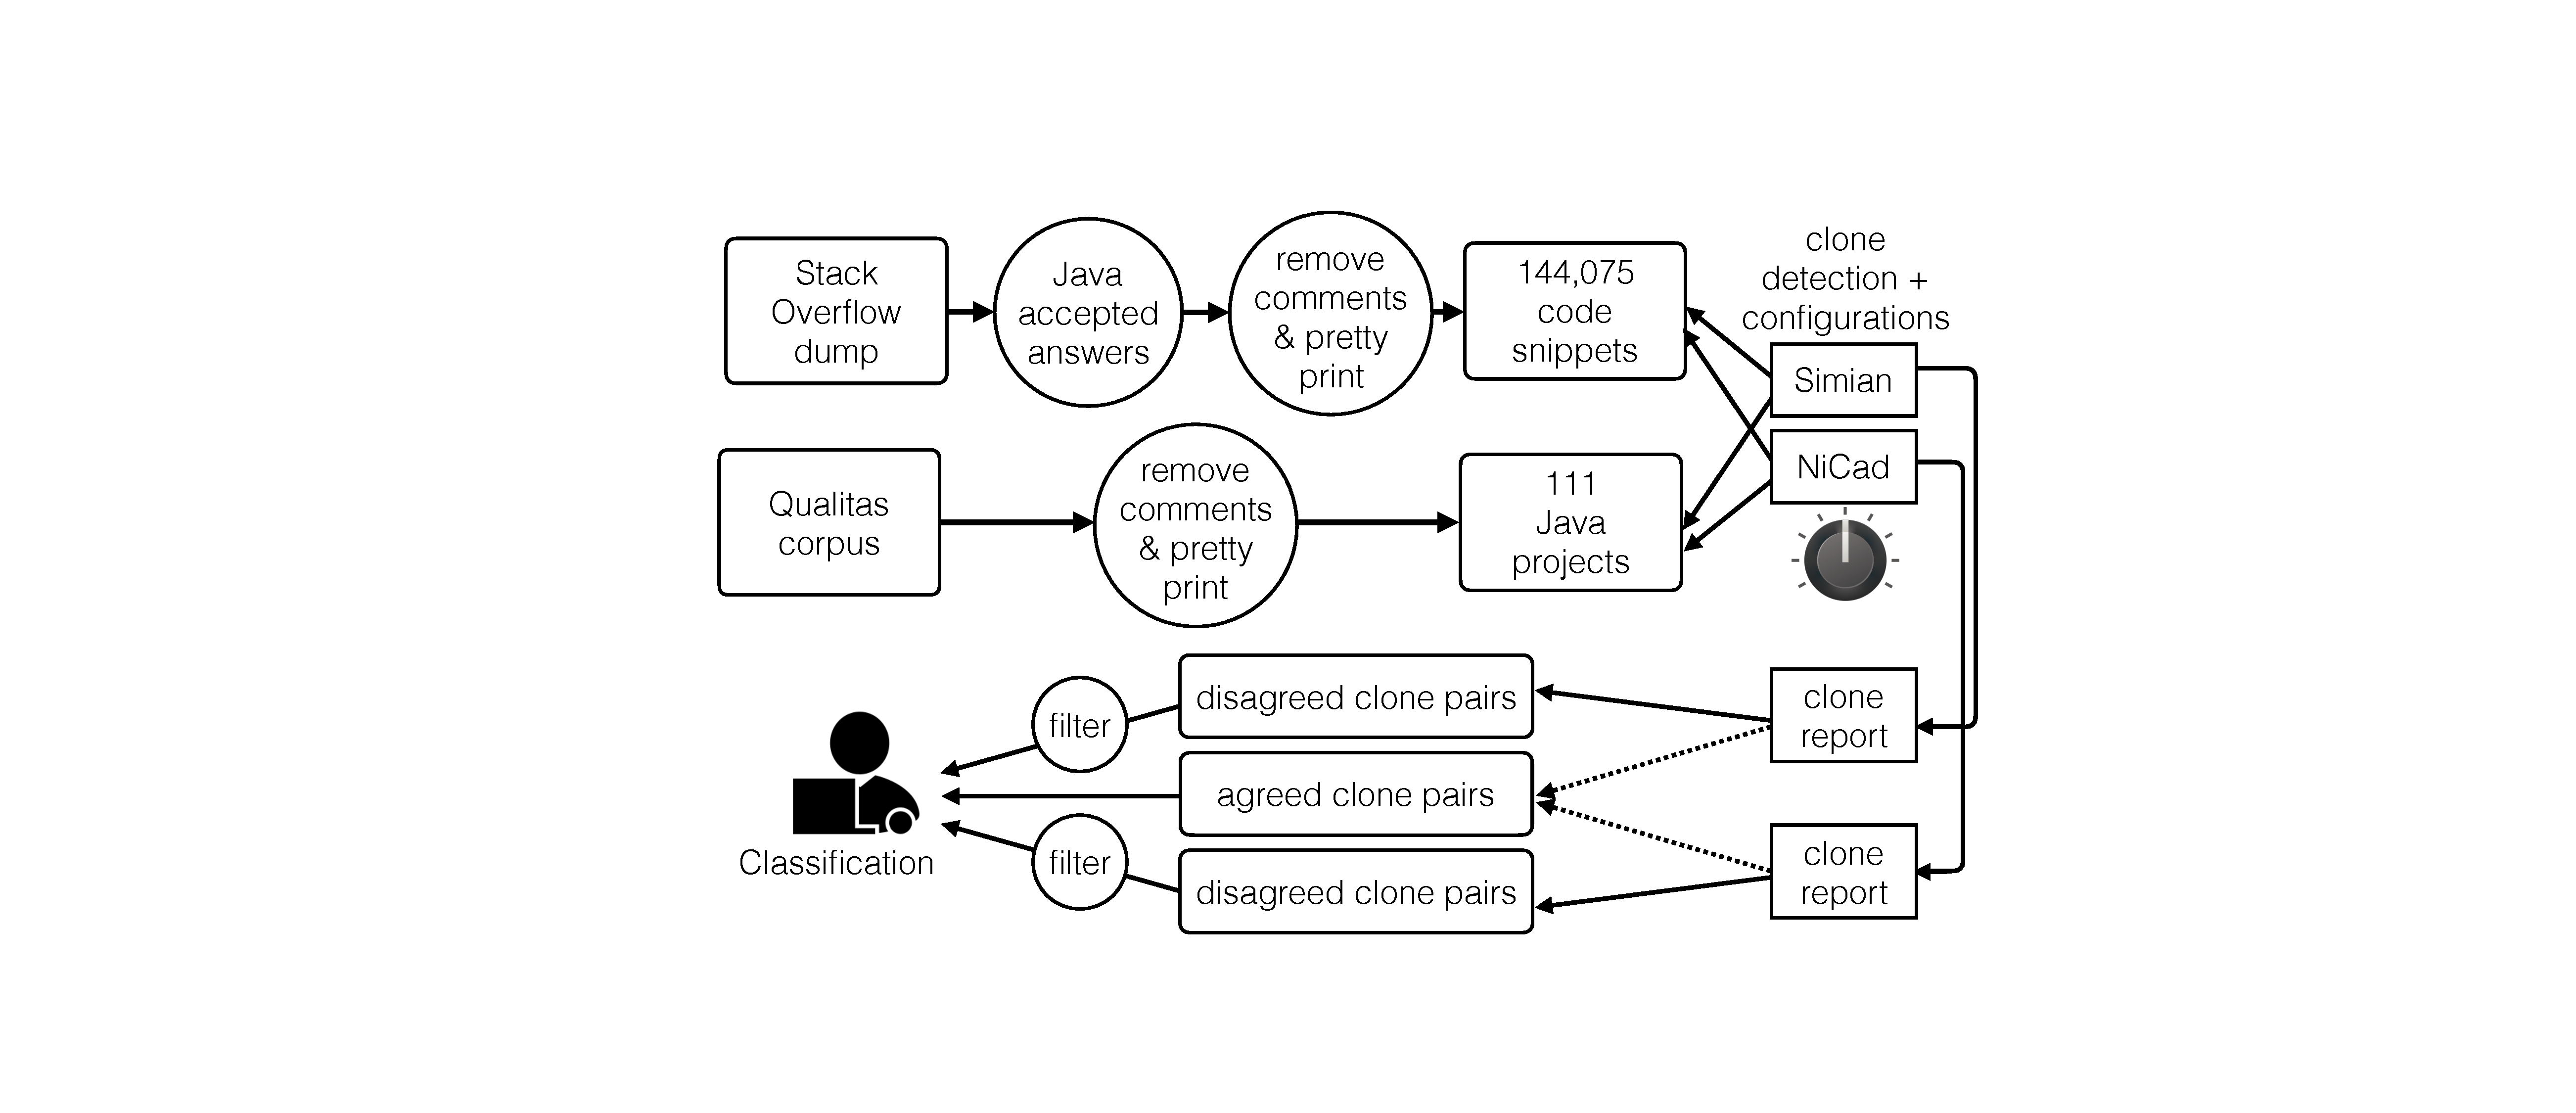
\includegraphics[width=\linewidth]{exp_framework_new}
  \caption{Experimental framework}
  \label{fig:exp_framework}
\end{figure}

%\subsection{Experimental Setup}
%\vspace{1ex}
To answer these four research questions, we perform an empirical study to
locate and study the online code clones between Stack Overflow and open source
projects. 
%
%\subsection{Methodology}
%
We designed our study in 6 phases as depicted in \Cref{fig:exp_framework} where
we build different data sets to answer each of our four research
questions. 

\subsection{Phase 1: Clone Identification}

We rely on two source data sets in this study: Java code snippets in answers
on Stack Overflow and open source projects from the Qualitas corpus
\cite{QualitasCorpus}.

\textbf{Stack Overflow:} 
We extracted Java code snippets from a snapshot of a Stack Overflow
dump\footnote{\url{https://archive.org/details/stackexchange}} in
January 2016. 
% The archived dump has a size of 9 gigabytes. 
The data
dump is in XML format containing information of posts
(questions and answers) and 
% supporting data such as user accounts and timestamps of the posts.
we were interested in code snippets embedded
in posts which were located between
{\small\texttt{<code>}...\texttt{</code>}} tags. A Stack Overflow
thread contains a question and several answers. An answer can also be
marked as \textbf{accepted answer} by the questioner if the solution
fixes his/her problem. We collected Java code snippets using two
criteria. First, we only focused on code snippets in accepted
answers. We chose the snippets in accepted answers because they
actually solved the problems in the questions. Moreover, they are
always displayed just below the questions which makes them more
likely to be reused than other answers. Second, we were only
interested in code snippets of at least six lines. Snippets smaller
than six lines are usually spurious clones~\cite{Bellon2007}. Each
snippet was extracted from the dump and saved to a file.
%using its post ID as the file's name. If an accepted answer had more than one code snippet, we appended an indexing number, starting from zero, after the post ID (e.g. 45051109\_0, and 45051109\_1.). Lastly, we added {\small\texttt{.java}} extension to the file's names so that clone detectors could recognise them. 
We obtained 144,064 Java code snippets containing 2,332,940
lines\footnote{Measured by cloc:
  \url{https://github.com/AlDanial/cloc}} of Java source code.
The median of the snippet size is 10.
% excluding comments and blank lines.

\textbf{Open source systems: }
We selected the established \textbf{Qualitas} corpus~\cite{QualitasCorpus} 
for this study. It is a curated Java corpus that has been used in several
software engineering
studies~\cite{Taube-Schock2011,Beckman2011,Vasilescu2011,Omar2012}. The
projects in the corpus represent various domains of software systems
ranging from programming languages to
visualisation. We selected the 20130901r release
of the Qualitas corpus containing 112 Java open source projects. This
release contains projects with releases no later than 1st September
2013. We intentionally chose an old corpus from 2013 since we are interested in
online code clones in the direction from open source projects to Stack
Overflow. The 20130901r snapshot provides Java code that is more than
2 years older than the Stack Overflow snapshot, which is sufficiently
long for a number of code snippets to be copied onto Stack Overflow
and also to observe if clones become outdated. Out of 112 Qualitas
projects, there is one project, \textsf{jre}, that does not contain
Java source code due to its licensing limitation~\cite{QualitasCorpus}
and is removed from the study. This resulted in a total of 111
projects analysed in the study. As shown in \Cref{tab:datasets}, the
111 Qualitas project have 166,709 Java files containing 19,614,083
lines of code. The median project size is 60,667 lines of code.

\begin{table}
  \centering
  \caption{Stack Overflow and Qualitas datasets}
  \label{tab:datasets}
  %\small
  \begin{tabular}{lrrr}
    \hline 
    Dataset & No. of files & SLOC & Median \\
    \hline
    Stack Overflow & 144,064 & 2,332,940 & 10 \\ 
    %\hline 
    Qualitas &  166,709 & 19,614,083 & 60,667 \\ 
    \hline 
  \end{tabular} 
\end{table}

\textbf{Clone Detection Tools: }
We use clone detection to discover online code clones. 
%\textbf{Clone Detection and Configuration: } 
There are a number of restrictions in terms of choosing the clone
detection tools for this study. The main restriction is due to nature
of code snippets posted on Stack Overflow, as most of them are
incomplete Java classes or methods. Hence, a detector must be flexible
enough to process code snippets that are not compilable or not
complete blocks. Moreover, since the amount of code that has to be
processed is in a scale of millions line of code (as shown in
\Cref{tab:datasets}), a clone detector must be scalable enough to
report clones in a reasonable amount of time. We have tried 5
state-of-the-art clone detectors including Simian~\cite{simian},
NiCad~\cite{Cordy,Roy2008}, CCFinder~\cite{Kamiya2002},
iClones~\cite{Gode2009}, and DECKARD~\cite{Jiang2007a} against the
Stack Overflow and Qualitas datasets. CCFinder, iClones, and DECKARD
failed with execution errors after running for couple of hours. Thus,
we removed them from the study. Simian and NiCad are flexible enough
to handle code with incomplete methods or classes and successfully
completed the detection.

\textbf{Simian} is a text-based clone detector that locates clones at
line-level granularity and has been used extensively in several clone
studies~\cite{Ragkhitwetsagul2016, Wang2013, Mondal2011, Cheung2015,
  Krinke2010}.
% It is a command-line tool which enables us to automate the
% detection. 
Furthermore, it offers normalisation of variable names and literals
(strings and numbers) which enables Simian to detect literal clones
(type-1) and parameterised clones (type-2). \textbf{NiCad} is also a
text-based clone detector which detects clones at either method- or
block-level granularity. It can detect clones of type-1, -2 up to
type-3 (clones with added and removed statements) and has
also been used in several empirical clone studies~\cite{Roy2008,
  Ragkhitwetsagul2016, Svajlenko2014, Wang2013, Mondal2011,
  Sajnani2016}. It utilises TXL~\cite{Cordy2006} for parsing and
pretty-printing source code and provides code normalisation by
variable renaming and abstraction. We use a variant of NiCad called
\textit{nicadcross}. It offers the same functionalities as the
original NiCad but is specialised for detecting code clones between
two systems. 
% NiCad is also a command-line tool which makes it suitable for
% automation.

%We processed two datasets, 144,064 Java code snippets from accepted answers on Stack
%Overflow and 111 open source projects from the Qualitas corpus. 
%The Java code snippets were extracted from Stack Overflow posts. 
We prepared the Java code in both datasets by removing comments and
pretty-printing to increase the clone detection accuracy. Then, we
deployed the two detectors to locate clones between the two
datasets.  For each Qualitas project, we ran the tools on the
project's code and the entire Stack Overflow data.
% For scalability reasons, we partitioned the input and ran the tools
% multiple times. Each run was composed of the entire Stack Overflow
% data and a single Qualitas project. We repeated the process until we
% covered all 111 projects.
% We then converted the clone reports to the General
% Clone Format (GCF)~\cite{Wang2013} and combined the 111 reports into a
% single GCF file.  
Simian did not provide an option to detect cross-project
clones. % between two locations.
Hence the Simian clone report was filtered to contain only clone pairs
between Stack Overflow and Qualitas projects, removing all clone pairs
within either Stack Overflow or within Qualitas.
% NiCad provides an option to detect clones
% from two locations so no filtering was needed.

\begin{table}
  \centering
  \caption{Configurations of Simian and NiCad}
  \label{t:param_tuning}
  %	\resizebox{\columnwidth}{!}{%
  \small
  \begin{tabular}{p{0.7cm}|p{2.4cm}p{3.8cm}}
    \hline 
    Tool & Default (\textit{D}) & EvaClone (\textit{E}) \\
    \hline
    Simian\newline (\textit{S}) &  threshold=6,\newline ignoreStringCase, \newline ignoreCharacterCase, \newline ignoreModifiers & threshold=5, ignoreIdentifiers, \newline ignoreIdentifierCase, \newline ignoreStrings, ignoreCharacters,\newline ignoreSubtypeNames, \newline balanceSquareBrackets \\ 
    \hline 
    NiCad\newline (\textit{N}) & Blocks, UPI=0.30,\newline MinLine=10,\newline MaxLine=2500 & Blocks, UPI=0.20, \newline MinLine=5, MaxLine=604, \newline blind renaming, literal abstraction \\
    \hline
  \end{tabular} %
%}
\end{table}

\textbf{Clone Detection Configuration: }
We are aware of effects of configurations to clone detection results
and the importance of searching for optimised configurations in
empirical clone
studies~\cite{Svajlenko2014,Wang2014,cr2016ssbse,Ragkhitwetsagul2016}. However,
considering the massive size of the two datasets and the search space
of at least 15 Simian and 5 NiCad parameters, we are unable to search
for the best configurations of the tools. Thus, we decided to
configure Simian and NiCad using two established configurations:
(1)~the tools' default configurations chosen by the tools' creators
(denoted as \textit{D}), and (2)~the discovered configurations for
Bellon's Java projects from \textit{EvaClone}~\cite{Wang2013}, a study
of optimising clone detectors' configurations based on clone agreement
(denoted by \textit{E}). \Cref{t:param_tuning} shows the two configurations.
In total, we have four configurations: Simian with the default
configuration ($S_D$), Simian with the EvaClone configuration ($S_E$), 
NiCad with the default configuration ($N_D$)
and NiCad with the EvaClone configuration ($N_E$).

We encountered NiCad failures with a few Qualitas projects.~$N_D$
could not detect clones in \textsf{hibernate} due to clustering
errors. $N_E$ generated errors during code normalisation for 5
projects including \textsf{vuze}, \textsf{hibernate},
\textsf{myfaces}, \textsf{netbeans}, and \textsf{spring}. We have
contacted the creator of NiCad regarding the issues. They identified
the issues as problems in the TXL grammar and as problems of long file
paths, and will be fixed in the next NiCad releases.

The number of online clone pairs reported % by running Simian and NiCad
are presented in \Cref{tab:orig_stats}. $S_D$ reports 67,570 clone
pairs while $N_D$ reports 632,855 clone pairs. $S_E$ and $N_E$ report
much larger numbers of clone pairs, 63,635,844 and 251,449,849 pairs
respectively. This is expected since EvaClone configurations prefer
recall~\cite{Wang2013}.  The average clone size reported by $S_D$ is
9.11 lines which is bigger than for $S_E$ (5.95 lines). Similarly,
$N_D$ has an average clone size of 10.85 lines which is bigger than
6.28 lines reported by $N_E$. The drop in size is due to the EvaClone
configuration with a smaller minimum size (\Cref{t:param_tuning}).

\begin{table}
	\centering
	\caption{Number of online clones reported by Simian (\textit{S}) and NiCad (\textit{N}) with default (\textit{D}) and EvaClone (\textit{E}) configurations}
	\label{tab:orig_stats}
	%\small
	%\resizebox{\columnwidth}{!}{%
	\begin{tabular}{l|r|r|r|r}
		\hline
		Stats & \multicolumn{1}{c|}{$S_D$} & \multicolumn{1}{c|}{$S_E$} & \multicolumn{1}{c|}{$N_D$} & \multicolumn{1}{c}{$N_E$} \\
		\hline
		Total C$_{\textrm{\textit{pairs}}}$ & 67,570 & 63,635,844 & 632,855 & 251,449,849 \\
		% Avg.~C$_{\textrm{\textit{pairs}}}$ & 62 & 41,565 & 455 & 19,356 \\
		Avg.~C$_{\textrm{\textit{size}}}$ & 9.11 & 5.95 & 10.85 & 6.28 \\
		\hline
	\end{tabular} %
	%}
\end{table}

\subsection{Phase 2: Clone Filtering}
As there are in total 315,786,118 clone pairs reported, it is
infeasible for humans to manually validate them all. Instead of
investigating a random sample, we adopted the idea of \textbf{clone
  agreement} which has been used in clone research
studies~\cite{Funaro2010, Wang2013,cr2016ssbse} in situations where a
clone oracle is missing or impossible to establish. Clone pairs agreed
by multiple clone detection tools have a higher likelihood to be real
clones~\cite{cr2016ssbse}. By using this agreement-based approach, we
reduced the number of clone candidates for manual investigation to the
ones agreed by multiple tools. To find agreement between two clone
pairs reported by two different tools, we used the clone pair matching
metric proposed by Bellon et al.~\cite{Bellon2007}. Two clone pairs
which have a large enough number of overlapping lines can be
categorised as either a good-match or an ok-match pair (denoted as
\textit{good} and \textit{ok} respectively) with a confidence value
between 0 and 1. A \textit{good} clone pair has stronger agreement
than an \textit{ok} pair. We follow the original definitions of good-
and ok-match introduced in Bellon's paper~\cite{Bellon2007}.

Given that a clone pair \textit{CP} is formed by two clone fragments
\textit{CF$_1$} and \textit{CF$_2$}, i.e.~\textit{CP} = (\textit{CF$_1$},
\textit{CF$_2$}), we can define the \textit{overlap}\footnote{The overlap value can be considered as Jaccard similarity.} and
\textit{contained} value of two clone pairs as
%\squeezeup
\begin{displaymath}
  overlap(\textrm{\textit{CP}}_1, \textrm{\textit{CP}}_2) = \frac{|lines(\textrm{\textit{CF}}_1) \cap lines(\textrm{\textit{CF}}_2)|}{|lines(\textrm{\textit{CF}}_1) \cup lines(\textrm{\textit{CF}}_2)|} 
\end{displaymath}
% \squeezeup
\begin{displaymath}
  contained(\textrm{\textit{CP}}_1, \textrm{\textit{CP}}_2) = \frac{|lines(\textrm{\textit{CF}}_1) \cap lines(\textrm{\textit{CF}}_2)|}{|lines(\textrm{\textit{CF}}_1)|}
\end{displaymath}
      
\noindent%
The \textit{good-value}  and the \textit{ok-value}  of two clone pairs are defined as
%\squeezeup
\begin{align*}
	good(\textrm{\textit{CP}}_1, \textrm{\textit{CP}}_2) = min(overlap(\textrm{\textit{CP}}_1.\textrm{\textit{CF}}_1,\textrm{\textit{CP}}_2.\textrm{\textit{CF}}_1), \\ overlap(\textrm{\textit{CP}}_1.\textrm{\textit{CF}}_2,\textrm{\textit{CP}}_2.\textrm{\textit{CF}}_2))
\end{align*}
\begin{align*}
	ok(\textrm{\textit{CP}}_1,\textrm{\textit{CP}}_2) = min(max(contained(\textrm{\textit{CP}}_1.\textrm{\textit{CF}}_1,\textrm{\textit{CP}}_2.\textrm{\textit{CF}}_1),~~ \\ contained(\textrm{\textit{CP}}_2.\textrm{\textit{CF}}_1,\textrm{\textit{CP}}_1.\textrm{\textit{CF}}_1)),~
	\\ max(contained(\textrm{\textit{CP}}_1.\textrm{\textit{CF}}_2,\textrm{\textit{CP}}_2.\textrm{\textit{CF}}_2),~~ \\contained(\textrm{\textit{CP}}_2.\textrm{\textit{CF}}_2,\textrm{\textit{CP}}_1.\textrm{\textit{CF}}_2)))
\end{align*}

\noindent%
Two clone pairs $\textrm{\textit{CP}}_1$ and $\textrm{\textit{CP}}_2$
are called a \textit{\textit{good-match}(t)} or \textit{ok-match(t)}  iff, for threshold $t \in [0,1]$ holds 
%\squeezeup
\begin{align*}
good(\textrm{\textit{CP}}_1,\textrm{\textit{CP}}_2) & \geq t\\
ok(\textrm{\textit{CP}}_1,\textrm{\textit{CP}}_2) & \geq t
\end{align*}

Using the good- and ok-match criteria with a predefined threshold
\textit{t}, we can prune the 315 million candidate clone pairs for
manual investigation. The \textit{good} pairs are the ones with the
highest confidence, followed by the \textit{ok} pairs, and followed by
clone pairs without agreement. We call the \textit{good}- and
\textit{ok}- pairs \textbf{agreed} clone pairs and the clone pairs
reported by Simian or NiCad without agreement \textbf{disagreed} clone
pairs.

Having two clone detectors, Simian (denoted as \textit{S}) and NiCad
(denoted as \textit{N}), with two chosen configurations (\textit{D}
and \textit{E}) each, we used Bellon's good- and ok-match for agreement
in four possible pair-wise combinations: $S_{D}$--$N_{D}$,
$S_{D}$--$N_{E}$, $S_{E}$--$N_{D}$, and $S_{E}$--$N_{E}$. %as shown in \Cref{t:param_tuning}.

\textbf{Agreed clone pairs: } As shown in \Cref{t_agreed_good_clone_pairs}, after we applied clone
agreement filtering using Bellon's criteria\footnote{Similar to the
  original study, we selected a threshold of 0.7 for
  \textit{good} and \textit{ok} pairs~\cite{Bellon2007}.}, the number
of \textit{good} clone pairs is 2,313 and the number of \textit{ok}
clone pairs is 32,316, 0.1\textperthousand~of all reported clone
pairs.  Agreed clone pairs are clone pairs that pass Bellon's
\textit{good} or \textit{ok} criteria, and therefore are selected for
manual classification.  Due to NiCad's failures, we do not have NiCad
clones from five Qualitas projects in the agreed clone pairs. Simian
clones of the same projects also disappeared from the agreed clone
pairs since they could not be matched.

\begin{table}
  \centering
  \caption{Distribution of the agreed clone pairs}
  \label{t_agreed_good_clone_pairs}
  %\small
  %	\resizebox{\columnwidth}{!}{%
  \begin{tabular}{l|r|r|r|r|r}
    \hline
    Set & $S_D$--$N_D$ & $S_D$--$N_E$ & $S_E$--$N_D$ & $S_E$--$N_E$ & Unique \\
    \hline
    \textit{good} & 23 & 26 & 10 & 2,267 & 2,313 \\
    \textit{ok} & 12,336 & 993 & 79 & 20,021 & 32,316 \\
    \hline
  \end{tabular} %
  % }
\end{table}

\begin{figure}
	\centering
	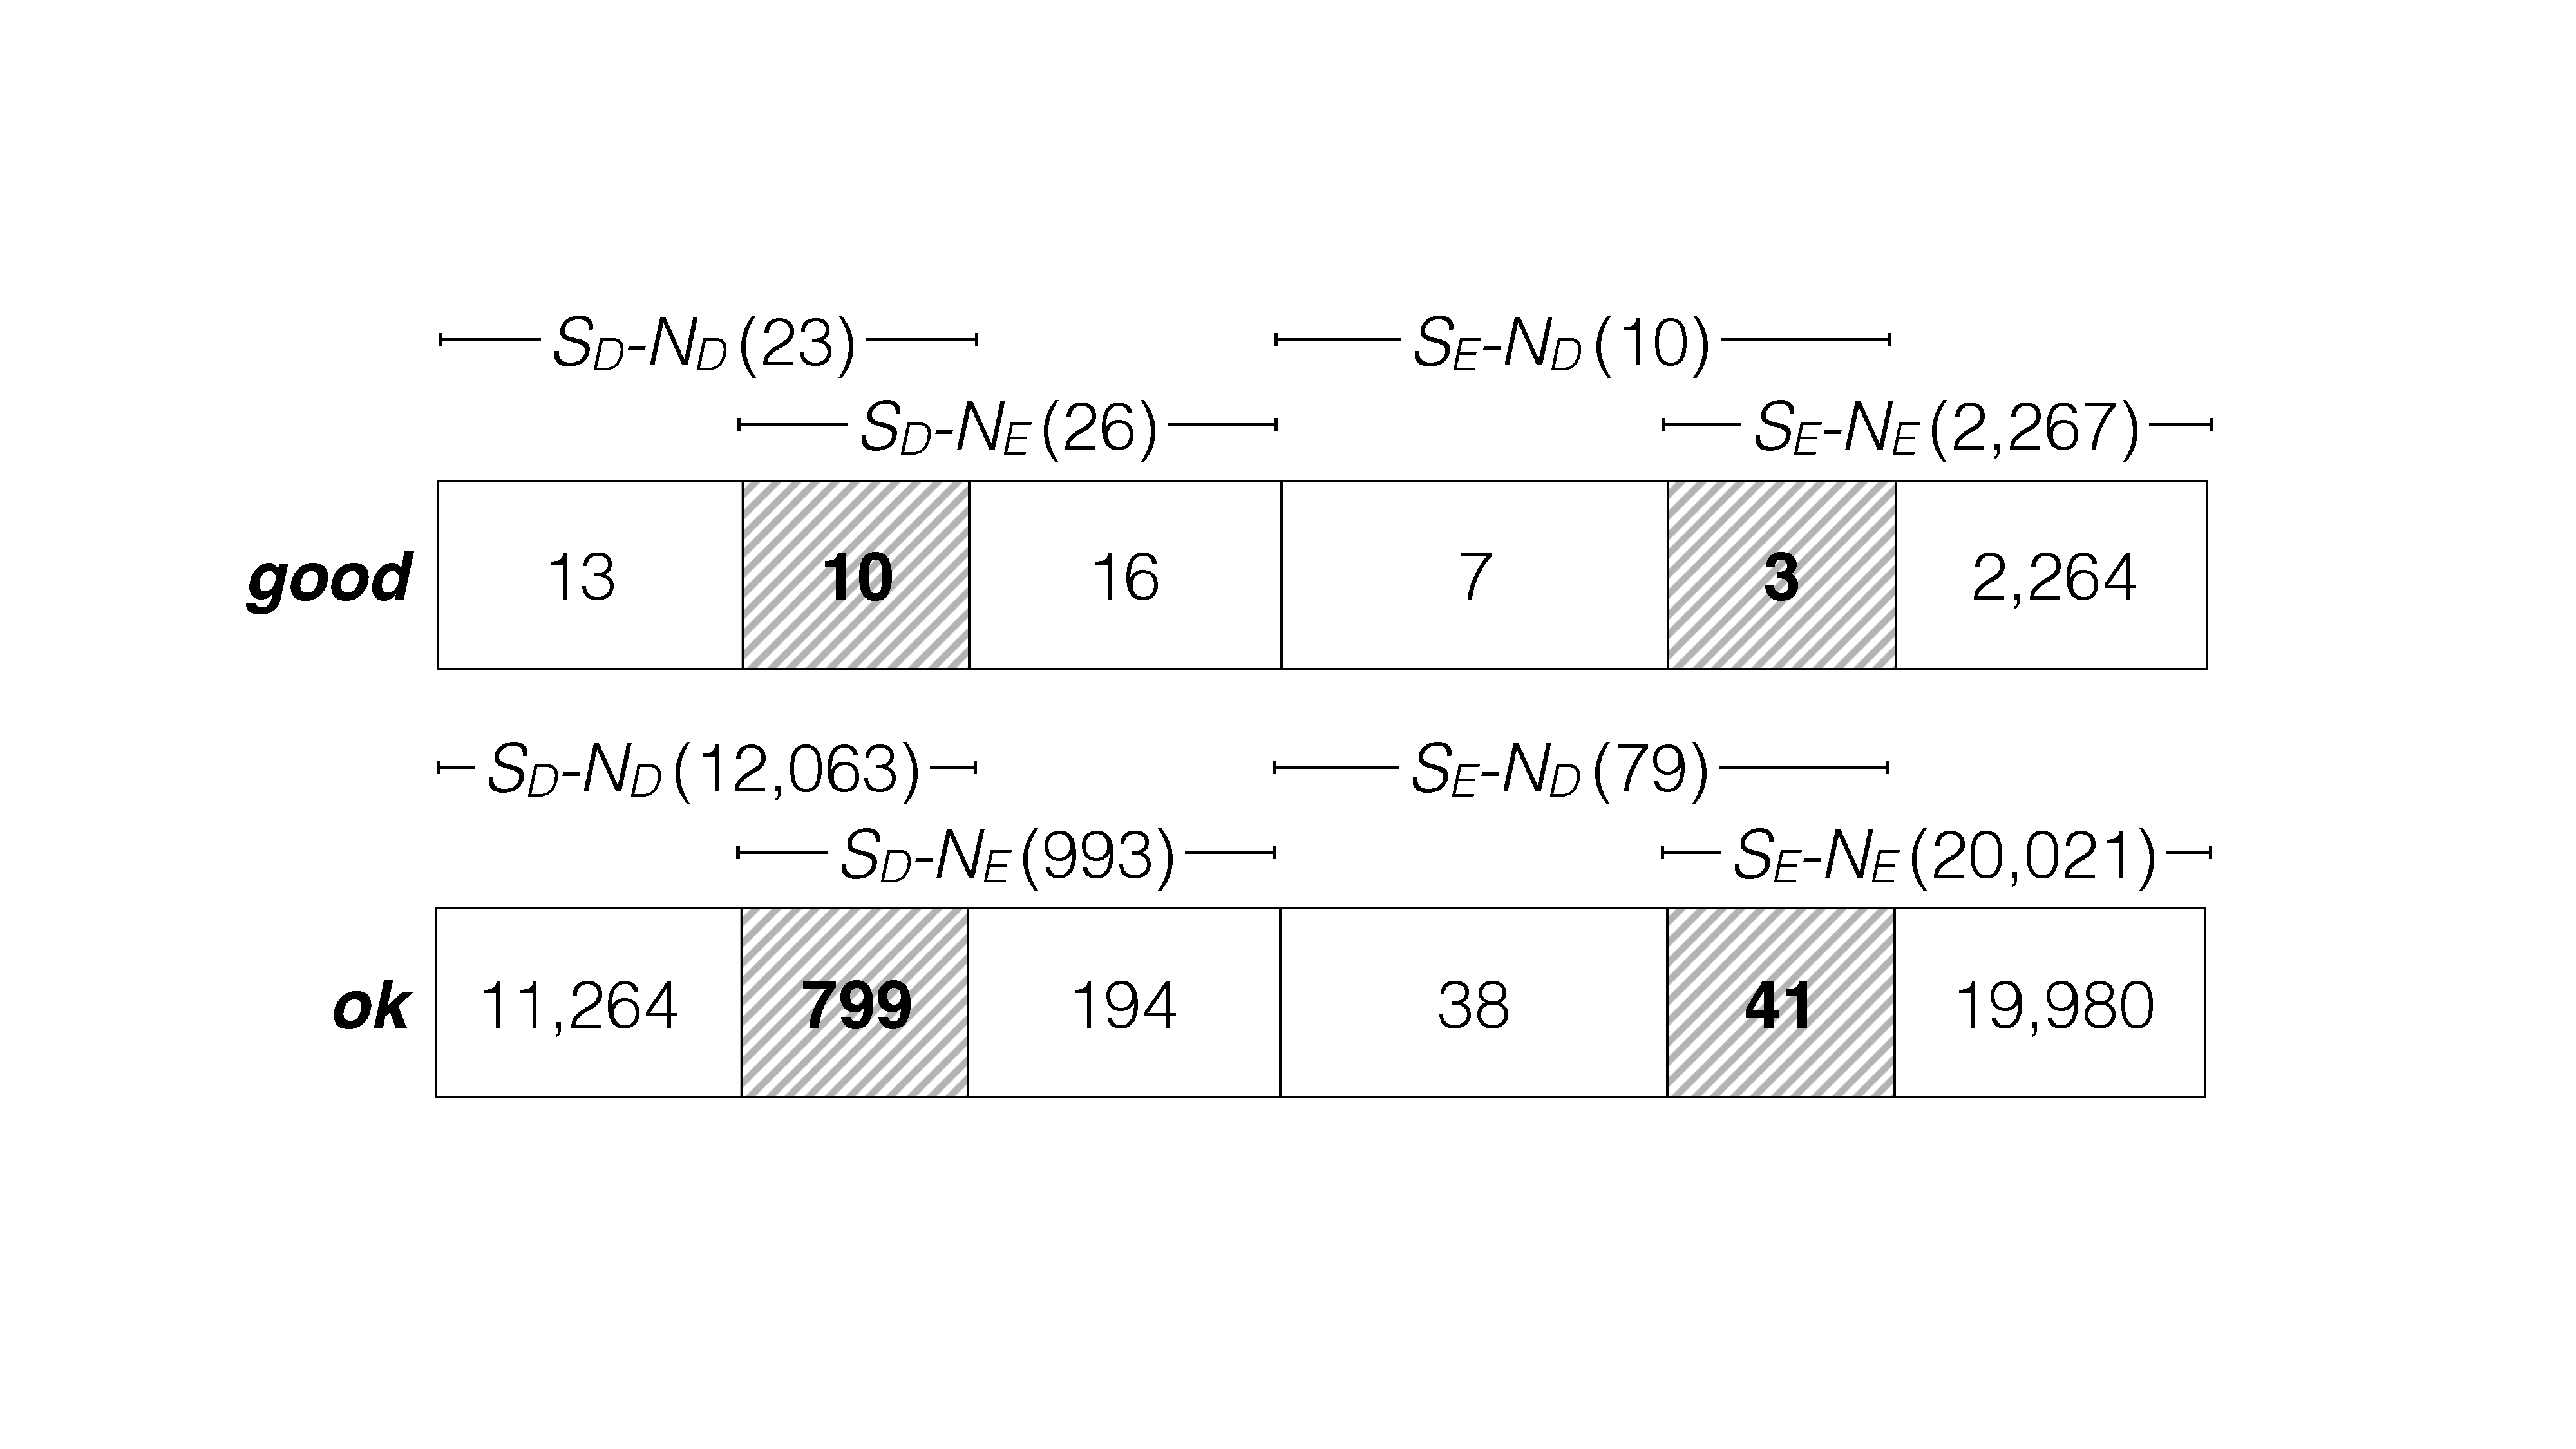
\includegraphics[width=0.9\linewidth]{good-ok_pairs}
	\caption{Distribution of \textit{good} (top) and \textit{ok} pairs (bottom) reported by the 4 configurations of Simian and NiCad. The shaded areas are overlapping pairs.}
	\label{fig:good-ok-pairs}
\end{figure}

The distribution of \textit{good} clone pairs between the four
combinations of \textit{D} and \textit{E} configurations are listed in
\Cref{t_agreed_good_clone_pairs}.  There are 2,326 (2,313 unique)
\textit{good} pairs consisting of 23 pairs from $S_D$--$N_D$, 26 pairs
from $S_D$--$N_E$, 10 pairs from $S_E$--$N_D$, and 2,267 pairs from
$S_E$--$N_E$. There are 33,156 (32,316 unique) \textit{ok}
pairs\footnote{This excludes the subsumed 2,313 \textit{good}
  pairs because \textit{ok} pairs subsume
  \textit{good} pairs.}. We obtained 12,336; 993; 79; and 20,021 pairs
from $S_D$--$N_D$, $S_D$--$N_E$, $S_E$--$N_D$, and $S_E$--$N_E$
respectively. Between the four configuration sets, there is
considerable amount of clone pairs shared between two adjacent sets
(as depicted in \Cref{fig:good-ok-pairs}), but there is no clone pair
that is agreed by all four combinations.

\begin{table}
	\centering
	\caption{Disagreed clone pairs before and after filtering.}
	\label{tab:online_clone_pairs}
	%\small
	%	\resizebox{\columnwidth}{!}{%
	\begin{tabular}{l|r|c|c|c|r}
		\hline
		\multirow{2}{*}{Set} & \multirow{2}{*}{Before Filtering} & \multicolumn{3}{c|}{Filters*} & \multirow{2}{*}{After Filtering} \\ \cline{3-5}
		& & \textit{L} & \textit{S} & \textit{G} & \\
		\hline 
		\multirow{1}{*}{$S_D$} & 67,570 & \checkmark & & \checkmark & 17,801 \\
		\multirow{1}{*}{$N_D$} & 632,855 & \checkmark & \checkmark & \checkmark & 83 \\ 
		\hline
		\multicolumn{6}{l}{*\textit{L}=size $\geq 10$, \textit{S}=sim $\geq 85\%$, \textit{G}=\textit{good}/\textit{ok} pairs.}  \\
	\end{tabular} %
	%}
\end{table}

\textbf{Disagreed clone pairs: }
The disagreed clone pairs are clone pairs that are reported by a
single tool, either Simian or NiCad, and do not have agreement with
the other tool. The disagreement can be from a misalignment of clone
lines or completely non-overlapping clones. The disagreed pairs from
Simian include clone pairs in the projects with NiCad's errors (1
project from $N_D$ and 5 from $N_E$).  With the four configuration
combinations, we decided to investigate only $S_D$, and $N_D$, and
dropped $S_E$ and $N_E$ due to their enormous amount of clone pairs
(60 and 250 millions respectively). Moreover, $S_E$ and $N_E$ contain
a large number of false positives due to the recall preference of
their EvaClone configurations.

Even choosing only the default configurations, the number of disagreed
clone pair candidates is still too large for manual inspection (67,570
for $S_D$ and 632,855 pairs for $N_D$). We applied three filters: clone
size, similarity threshold, and good/ok pairs. For
the \emph{clone size filter}, we raised the minimum clone size to 10 lines
since larger clones are more interesting, while smaller ones tend to
be false clones~\cite{Saini2016}.
% Since the 10--line threshold is already the default configuration for
% NiCad, this filter is applied to Simian only (Simian's default
% configuration has a minimum clone size of 6 lines).
The second filter, \emph{similarity threshold}, applies
only to NiCad clone pairs since Simian does not provide a similarity
configuration. The last filter, \emph{good/ok pairs}, removes the
clone pairs that already exist in the agreed clone sets.

As shown in \Cref{tab:online_clone_pairs}, for $S_D$ we filtered the
results using clone size and gook/ok pairs. The
two filters reduced the number of $S_D$ clones to 17,801 pairs. We
filtered $N_D$ clones by additionally raising the similarity
threshold. We increased NiCad's similarity threshold from 70\% to 85\%
(by adjusting NiCad's $\mathrm{UPI}$ parameter from 0.3 to 0.15). We
tried varying the threshold from 70\% (default, 632,855 pairs), 80\%
(25,003 pairs), 85\% (185 pairs) and 90\% (83 pairs) and found that
85\% similarity provided the best balance in terms of the amount of
reported clones and precision for small clones. Using this filter
along with the other three filters, we reduced the number of $N_D$
clones to 83 pairs.

%\subsection{Filtered Clones Set}
We selected all \textit{good} pairs (2,313) and the \textit{ok} pairs for
$S_D$--$N_D$ (12,336), $S_E$--$N_D$ (993), and $S_D$--$N_E$ (79), but we ignored
20,021 $S_EN_E$ \textit{ok} clone pairs in the classification due to
their large number of clones and the very small average clone sizes of
5.95 and 6.28 lines (see \Cref{tab:orig_stats}), leading to a high
probability of being trivial clones. We refer to the set of clone
pairs as the \textit{good} set and the \textit{ok'} set.
Together with the 17,801 (referred as $S_D'$ set) and 83 (referred as
$N_D'$ set) clone pairs after filtering, we ended up with a set of 32,533 online clone pair candidates.

Before performing the manual
investigation, we created and used an automatic classifier 
to classify boiler-plate code of {\small\texttt{equals()}}, 
{\small\texttt{hashCode()}} and getters/setters 
(depicted with a grey line in \Cref{fig:exp_framework}).
The classifier could automatically classify 28,897 clone pairs 
and left 3,636 clone pairs for manual investigation in phases 3 to 6.

\subsection{Phase 3-4: Validation and Classification}
We used the 3,636 filtered clone pairs after automatic classification for
manual validation and classification.
The validation and classification of the pairs was done at the same time. 
The clone validation process (phase 3 in \Cref{fig:exp_framework}) involves checking 
if a clone pair is a true positive or a false positive. 
Moreover, we are also interested in 
the patterns of code cloning so we can gain more insights into 
how these clones are created (phase 4 in \Cref{fig:exp_framework}). 

For manual investigation, the first author, who has been working on clone detection research for 
two years, took the role of the main investigator performing a manual 
validation and classification of the filtered clone pairs. 
%By consulting the cloning patterns, 
The main investigator went through each clone pair candidate, 
looked at the clones, and decided if they are a true positive or a
false positive and classified them into an appropriate pattern. 
%the most appropriate cloning pattern for the pair. 
To mitigate the human error of the manual investigation, 
the second author took the role of the validating investigator, performing a
validation on 10\% (364 pairs) of the clone pairs judged by the main
investigator. After the validation, the results from the two
investigators were compared and 61 conflicts were discussed and resolved.
There were 3 conflicts where the two investigators could not find a consensus 
and the third author was involved for the final judgement.

\textbf{The online cloning classification patterns:} 
We studied the 8 patterns of cloning from Kapser et
al.~\cite{Kapser2006,Kapser2008} and performed a preliminary study to
evaluate its applicability to our study. 
We tried to classify 697 online clone pairs from
the reported clones in phase 1 
%Using the $S_D$ clone report,
%snippets were ranked according to (1)~clone pair frequency,
%(2)~popularity (i.e.~number of associated Qualitas projects),
%(3)~clone size in SLOC, and (4)~ratio of cloned code per snippet. We
%selected these four criteria so that we could cover the online clones
%from various aspects. We selected the top 10 from each ranking and
%obtained 34 unique Stack Overflow snippets. The snippets were
%associated with 697 clone pairs.
%\subsection{Defining Online Code Cloning Patterns}
using Kapser's cloning patterns. We found that 
% the
% clone pairs were categorised into either Customisation or Templating.
% Thus, 
Kapser's patterns are too broad for our study and a
more suitable and fine-grained classification scheme is needed. After
the preliminary study, we adopted one of Kapser's cloning patterns,
\emph{boiler-plate code}, and defined
6 new cloning patterns. The seven patterns include QS, SQ, EX, UD, BP,
IN, and AC as presented in \Cref{tab:classification_scheme}. Pattern
QS (\textbf{Q}ualitas to \textbf{S}tack Overflow) represents clones
that have evidence of being copied from a Qualitas project to Stack
Overflow. The evidence of copying can be found in comments in the
Qualitas source code or in the Stack Overflow post's contents. Pattern
SQ (\textbf{S}tack Overflow to \textbf{Q}ualitas) is cloning, with
evidence, in the opposite direction from Stack Overflow to a Qualitas
project. Pattern EX (\textbf{Ex}ternal Sources) is cloning that has
evidence of copying from a single or multiple external sources to
Stack Overflow and to a Qualitas project.  Pattern UD
(\textbf{U}nknown \textbf{D}irection) is cloning that creates
identical or highly similar clones between Qualitas and Stack Overflow
but where we could not find any attribution of copying.
Pattern BP (\textbf{B}oiler-\textbf{P}late) represents clones
containing boiler-plate code of {\small\verb|equals()|} methods,
getters/setters, or IDE-generated code such as GUI components. Pattern
IN (\textbf{In}heritance/Interface) is cloning by inheritance of the
same super class or implementation of the same interface. These two
activities usually result in similar overriding methods. The last
pattern, AC (\textbf{A}ccidental \textbf{C}lones), represents
accidentally similar clone pairs. These are mainly false positive
clones from the clone detectors such as similar
{\small\texttt{try-catch}} statements.

\begin{figure}
	\centering
	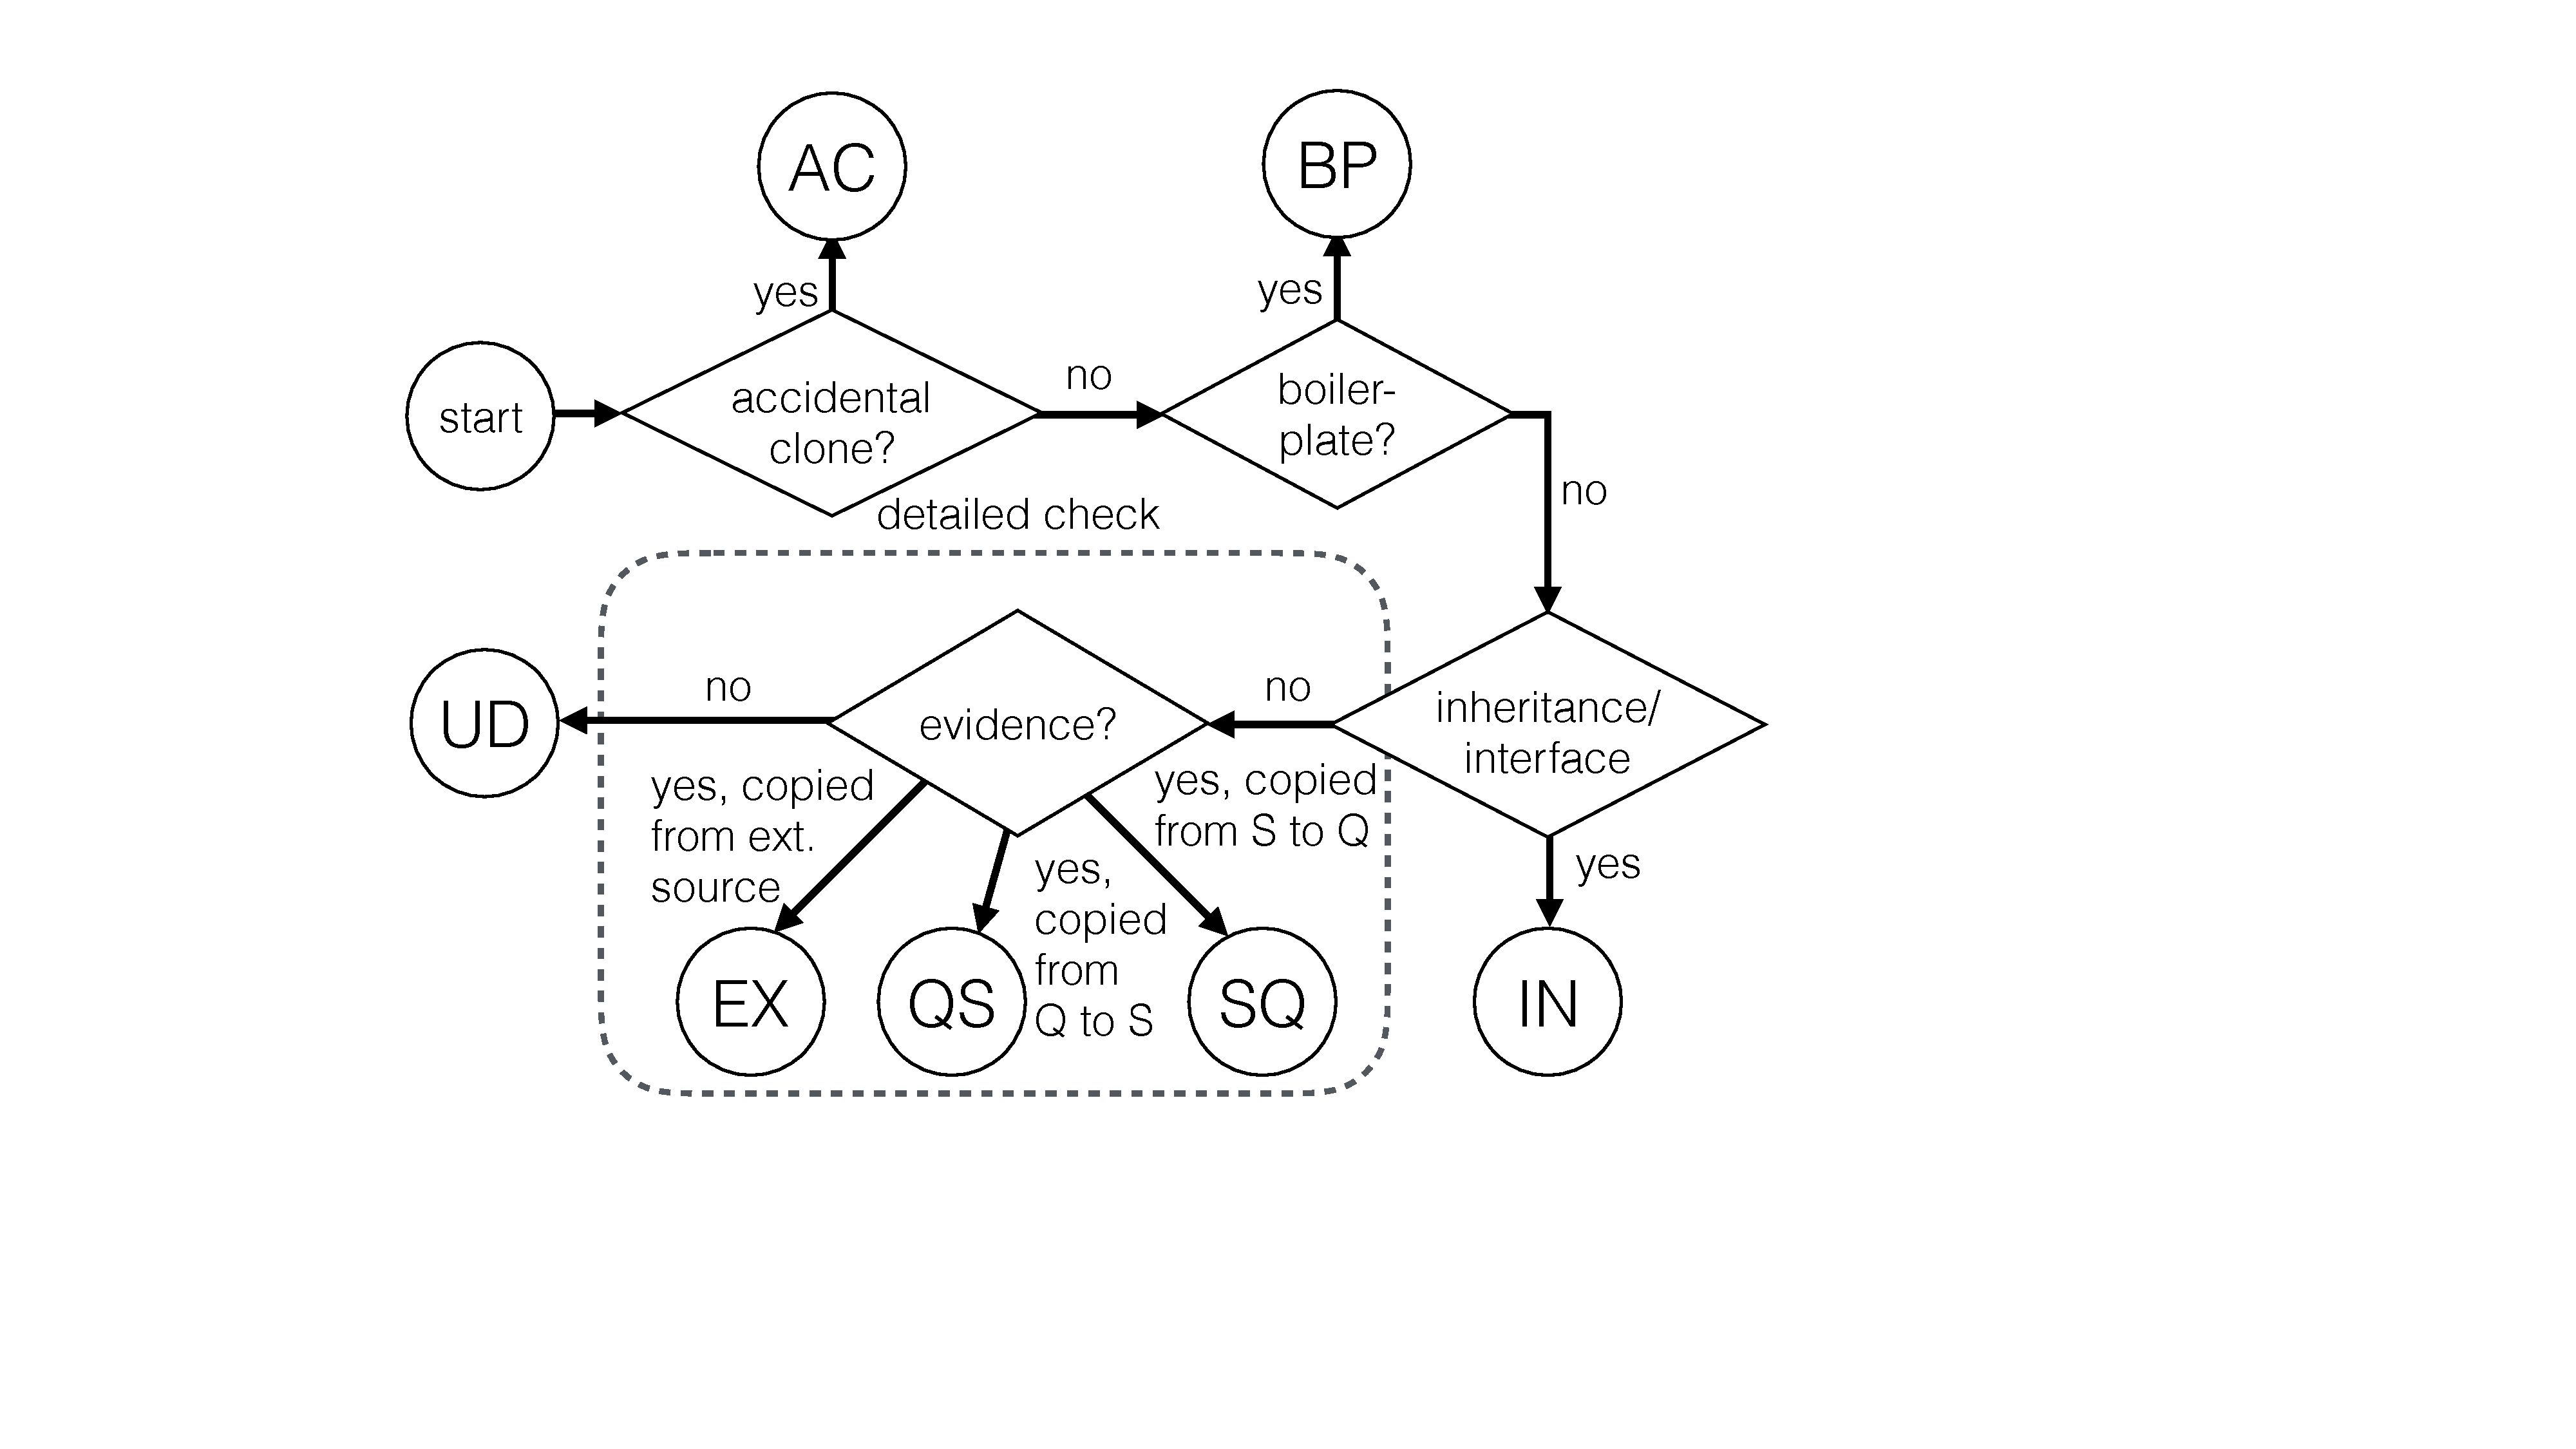
\includegraphics[width=0.8\linewidth]{classification_process}\vspace{-1ex}
	\caption{Online code clone classification process}
	\label{fig:classification_process}
\end{figure}

The classification of the filtered online clone pairs followed the steps
depicted in \Cref{fig:classification_process}. First, we look at a
pair of clone fragments to see their similarity. If they are
accidentally similar clones after code normalisation or false positive
clones from the clone detection tools, we classify the pair into
\textbf{AC}. If the two fragments are boiler-plate code, the pair is
classified into \textbf{BP}. If they implement the same interface or
inherited the same class and share similar overriding methods, the
pair is classified into \textbf{IN}. If the pair is not \textbf{BP},
\textbf{IN}, or \textbf{AC}, we start a detailed investigation. We
check the corresponding Stack Overflow post, read through it carefully
and look for any evidence mentioning code copying. If evidence of
copying has been found from a Qualitas project, the pair is classified
in \textbf{QS}. In several occasions, we used extra information such
as questions' contents, name of posters, and tags to gain a better
understanding. On the other hand, if the source code from the Qualitas
project mentions copying from Stack Overflow, the pair is classified
into \textbf{SQ}. If there is evidence of copying from an external
source instead of a Qualitas projects, the pair is classified into
\textbf{EX}.
Lastly, if there is no evidence of copying in any
direction but the clone fragments are highly similar, we classify them
into \textbf{UD}.

\begin{table}
	\centering
	\caption{The seven patterns of online code cloning}
	\label{tab:classification_scheme}
	%\resizebox{\columnwidth}{!}{%
        \small\vspace{-1ex}
		\begin{tabular}{c@{~~}p{7.35cm}}
			\hline 
			Patt. & Description \\ 
			\hline 
			QS & Cloned from Qualitas project to Stack Overflow (Q $\rightarrow$ S). \\ 

			SQ &Cloned from Stack Overflow to Qualitas project (S $\rightarrow$ Q). \\ 

			EX & Cloned from an external source \textit{X} (X $\rightarrow$ S $\wedge$ X $\rightarrow$ Q). \\

			UD & Cloned from each other or from an external source \textit{X} outside the project (unknown) (S $\leftrightarrow$ Q $\vee$ (X $\rightarrow$ S $\wedge$ X $\rightarrow$ Q)). \\ 
			\hline 
			BP & Boiler-plate or IDE auto-generated \\ 

			IN & Inheritance, interface implementation  \\ 

			AC & Accidental similarity, false clones \\ 
			\hline 
		\end{tabular}  %
	%}
\end{table}

\subsection{Phase 5: Outdated Clones}
Outdated code occurs when a piece of code has been copied from its
origin to another location and later the original has been
updated~\cite{Xia2014}. Usually code clone detection is used to locate
clone instances and update them to match with the
originals~\cite{Bellon2007}. However, online code clones are more
difficult to detect than in regular software projects due to its large
search space and a mix of natural and programming languages combined
in the same post.
%Moreover, Stack Overflow is not a software. There is no test suite to run and check whether the validity of the code snippets. To the best of our knowledge, this work is the first to address the problem of outdated code on Stack Overflow. 

To search for outdated online code clones, we focused on the
\textbf{QS} clone pairs that were cloned from Qualitas to Stack
Overflow and compared them with their latest versions. We downloaded
the latest version of the Qualitas projects from their repositories on
26 September 2016. For each \textbf{QS} online clone pair, we used the
clone from Qualitas as a proxy. We searched for its latest version by
the file name and located the cloned region in the file based on the
method name.
%For Simian clones, where clones may span across several methods, we scanned upwards until we find a method name ahead of the clone region. 
We then compared the Stack Overflow snippet to its latest version
line-by-line to find if any change has been made to the source
code. We also made sure that the changes did not come from the
modifications made to the Stack Overflow snippets by the posters but
from the updates in the projects themselves. When we found
inconsistent lines between the two versions, we used
{\small\texttt{git blame}} to see who modified those lines of code and
the timestamps.

\subsection{Phase 6: Licensing Analysis}
Software licensing plays an important role in software
development. Violation of software licenses impacts software delivery
and also leads to legal issues~\cite{Sprigman2015}.
%It is an emerging area that software engineering research community is paying attention to. For example, 
One can run into a licensing issue if one integrates third-party
source code into their software without checking. A study by An et
al.~\cite{An2017} reports 1,219 cases of potential license violations
between 399 Android apps and Stack Overflow code
snippets.

We analysed licensing conflicts of the online clones in the
\textbf{QS}, \textbf{EX}, and \textbf{UD} set. The
licenses were extracted by \emph{Ninka}, an automatic license
identification tool~\cite{German2010}. Since Ninka works at file
level, we report the findings based on Stack Overflow snippets and
Qualitas source files instead of the clone pairs (duplicates were
ignored). For the ones that could not be automatically identified by
Ninka and have been reported as {\small\texttt{SeeFile}} or
{\small\texttt{Unknown}}, we looked at them manually to see if any
license can be found. 

% The table shows the license mapping of Stack Overflow snippets and
% Qualitas source code. The results are reported separately for the
% \textbf{QS}, \textbf{EX}, and \textbf{UD} set.

%\subsection{Analysis Methods}

% We followed the 6 phases in the experimental framework (\Cref{fig:exp_framework})
% to answer our four research questions. 
% To answer RQ1, we rely on the number of manually validated true positive online clone pairs
% in phase 3. We use the results of the manual classification using the
% patterns of online code cloning to answer RQ2. 
% For RQ3, we looked at the true positive clone pairs that are classified 
% as cloned from Qualitas to Stack Overflow and
% checked if they have been changed since they have been
% cloned. Similarly, for RQ4, we looked at the license of each clone in the pattern 
% QS, EX, UD and checked for a possibility of a licensing violation.

%\subsection{Manual Investigation}
%We did not have an oracle of clones
%between the two data sets so we rely on a manual investigation to
%validate the reported clone candidates. However, the large amount of
%generated clone pairs hindered us from looking at all of them.
%A random sampling of clones could have been employed, however, the 
%risk of returning false positives non-meaningful clones is increased.
%Instead of extracting a random sample, we selected clone pair
%candidates by relying on \emph{agreement} of clone detectors. If a
%clone pair was reported by multiple tools, we had a higher
%confidence that it was a real clone pair. To achieve this, clone pairs
%from the two clone detectors were pair-wise matched to find agreements
%using Bellon's clone overlapping criteria~\cite{Bellon2007}. This step
%generated 
%\textbf{agreed clone pairs}. They were pairs with high confidence to be true clones since
%they obtained agreement from both tools. Then, pairs reported by
%Simian and NiCad that did not find agreement were categorised as
%\textbf{disagreed clone pairs}. The disagreed clone pairs were clones
%with less confidence than the agreed ones. 
%Finally, agreed and
%disagreed clone pairs have been looked at manually by two of the
%authors.

%In the manual inspection process, we classified clones into seven
%categories according to information observed from code comments and
%text in the Stack Overflow answer. This process took approximately a
%month until we successfully investigated 3,632 clone pairs. Clone
%pairs that were classified as false clones, boiler-plate code, or
%IDE-generated are not very interesting and were ignore in the analysis
%of outdated code and licensing violation. We compared the licensing
%information of the 668 remaining clone pairs for possibilities of software
%licensing violations. Moreover, we looked at the history starting at
%the date of the answers to today from its git repository. With this
%method, we discovered \textbf{outdated code}, i.e.~code that changes
%were made to them after they have been copied to Stack
%Overflow. 
%hence resulting in outdated clones on Stack Overflow.

\section{Results and Discussion}

We followed the 6 phases in the experimental framework (\Cref{fig:exp_framework})
to answer our four research questions. 
To answer RQ1, we rely on the number of manually validated true positive online clone pairs
in phase 3. We use the results of the manual classification by the
seven patterns of online code cloning to answer RQ2 (phase 4). 
For RQ3, we looked at the true positive clone pairs that are classified 
as clones from Qualitas to Stack Overflow and
checked if they have been changed after cloning (phase 5). Similarly, for RQ4, we looked at the license of each clone in the pattern 
QS, EX, UD and checked for a possibility of licensing violation (phase 6).

\subsection{RQ1: Online Code Clones} 

The statistics on clones obtained from the different data sets are
presented in \Cref{tab:snippets}. Simian in the default configuration
($S_D$) reported clones in 1,086 snippets, approximately 1\% of the
144,064 Stack Overflow snippets, associated with 92 Qualitas
projects. Simian in the EvaClone configuration ($S_E$) reported 1,531
snippets containing clones associated with all 111 Qualitas
projects. NiCad in the default configuration ($N_D$) reported clones
between 1,392 Stack Overflow code snippets and 88 Qualitas
projects. NiCad in the EvaClone configuration ($N_E$) reported the
largest number of 12,886 cloned snippets mainly due to the more
relaxed configuration. The $N_E$ snippets are associated with 88
Qualitas projects.  For the cloned Stack Overflow snippets, the
average ratio of cloned code for $S_D$, $S_E$, $N_D$, and $N_E$ is
38\%, 50\%, 30\%, and 33\% respectively.
% A quick manual check of Simian's clone report revealed that there
% were 11 problematic snippets. These 11 snippets triggered Simian to
% generate large clone clusters containing a huge number of false
% clones from array initialisation. Hence, their clones were removed
% from further analyses.

% \FIXME{Do you think we should report at this level or in more details 
% 	into $S_D$--$N_D$, $S_D$--$N_E$, $S_E$--$N_D$, $S_E$--$N_E$??}
% I don't think there is a need.

\begin{table}
\caption{Investigated online clone pairs and corresponding snippets
  and Qualitas projects for the different data sets}
\label{tab:snippets}
\centering
\begin{tabular}{l|rrrr}
  \hline 
  Data Set & Pairs & Snippets & Projects & Avg.~C$_{\textrm{\textit{\%}}}$ \\
  \hline 
  \multicolumn{5}{l}{\textit{Reported Clones}} \\
  \hline
  $S_D$ & 67,570 & 1,086 & 92 & 38\% \\
  $S_E$ & 63,635,844 & 1,531 & 111 & 50\% \\
  $N_D$ & 632,855& 1,392 & 88 & 30\% \\
  $N_E$ & 251,449,849& 12,886 & 88 & 33\% \\
  \hline
  Total & 315,786,118 & 14,856 & 111 & 38\% \\
  \hline
  \multicolumn{5}{l}{\textit{Filtered Data Set}} \\
  \hline
  \textit{good} & 2,313 & 97 & 67 & 23\% \\
  \textit{ok'} & 12,336 & 139 & 43 & 28\% \\
  $S_D'$ & 17,081 & 460 & 74 & 31\% \\
  $N_D'$ & 83 & 44 & 19 & 27\% \\
  \hline
  Total & 32,533 & 623 & 96 & 27\%\\
  \hline 
%  \multicolumn{5}{l}{\textit{Filtered Data Set without AC}} \\
%  \hline 
%  $\textit{good}/\textrm{AC}$ & 141 & 52 & 26 & 23\% \\
%  $\textit{ok'}/\textrm{AC}$ & 12,229 & 126 & 36 & 28\% \\
%  $S_D'/\textrm{AC}$ & 17,673 & 448 & 72 & 31\% \\
%  $N_D'/\textrm{AC}$ & 70 & 39 & 16 & 29\% \\
%  \hline
%  Total & 30,113 & 556 & 80 & 28\% \\
%  \hline
  \multicolumn{5}{l}{\textit{True Positives in Manually Validated Clones}} \\
  \hline 
  $\textit{good}/\textrm{AC}$ & 131 & 51 & 24 & 22\% \\
  $\textit{ok'}/\textrm{AC}$ & 152 & 83 & 22 & 21\% \\
  $S_D'/\textrm{AC}$ & 873 & 337 & 60 & 35\% \\
  $N_D'/\textrm{AC}$ & 60 & 33 & 15 & 27\% \\
  \hline
  Total & 1,216 & 516 & 75 & 26\% \\
  \hline
\end{tabular}
\end{table}

However, using Bellon's criteria for matching clone pairs, only
0.1\textperthousand~of all pairs are agreed by two tool/configuration
combinations. As shown in \Cref{tab:snippets}, for the 2,313
\textit{good} pairs, there are 97 Stack Overflow snippets which are
associated with 67 Qualitas projects. The 12,336 \textit{ok'} pairs
are clones between 139 Stack Overflow snippets and 43 Qualitas
projects.  Moreover, for the disagreed pairs, we found 17,081 clone
pairs reported by $S_D'$ are clones between 460 Stack Overflow
snippets and 74 Qualitas projects and 83 $N_D'$ clone pairs are clones
between 44 Stack Overflow snippets and 19 Qualitas projects. In total
we found that the filtered data sets contains 32,533 clone pairs which
are clones between 623 Stack Overflow snippets and 96 Qualitas
projects. 

During the manual investigation of 3,636 clone pairs, we identified 2,420 pairs
as being accidential clones (AC), i.e.~false positives. After removing
them, the set still contains 1,216 true positive clone pairs between 516 Stack
Overflow snippets and 75 Qualitas projects.

\textbf{To answer RQ1, we found most Qualitas projects to share
  similar code with Stack Overflow code snippets. In the manually confirmed 
  data set of 3,636 clone pairs, we found 1,216 pairs as true positives which 
  account for 75 Qualitas projects and
  516 Stack Overflow code snippets.}

%\FIXME{Should we have removed the AC clones right at the beginning?}

\subsection{RQ2: Patterns of Online Code Cloning}

\begin{table}
	\centering
	\caption{No.~of online clones candidates for the classification}
	\label{tab:online_clone_classification_results}
	%\small
	%	\resizebox{\columnwidth}{!}{%
	\begin{tabular}{l|r|r|r}
		\hline
		\multirow{2}{*}{Set} & \multirow{2}{*}{Candidates} & \multicolumn{2}{c}{Classification} \\ \cline{3-4}
		& & Auto & Manual \\
		\hline 
		\multirow{1}{*}{\textit{good}} & 2,313 & 10 & 2,303 \\
		\multirow{1}{*}{\textit{ok'}} & 12,336 & 12,077 & 259 \\
		%\multirow{1}{*}{\textit{agreed clone pairs}}      & 29,099 \\
		\multirow{1}{*}{$S_D'$} & 17,801 & 16,800 & 1,001 \\
		\multirow{1}{*}{$N_D'$} & 83 & 10 & 73 \\ 
		%\multirow{1}{*}{\textit{disagreed clone pairs}}    & 1,039 \\
		\hline
		Total  & 32,533 & 28,897 & 3,636 \\ 
		\hline
	\end{tabular} %
	%}
\end{table}

As shown in \Cref{tab:online_clone_classification_results}, the automatic
classifier helped us to classify 28,897 clone pairs into
pattern \textbf{BP}. Then, we relied on a manual classification
% to qualitatively investigate the patterns of
%online code cloning 
on the remaining 3,636 pairs by following the classification process
in \Cref{fig:classification_process}. 
%To achieve this, we classified all 32,533
%selected clone pairs according to the classification process 
%in \Cref{fig:classification_process}.  
%
%There were 3,636 pairs left for the manual check. 
The classification results are shown in \Cref{tab:classification_good_o} 
and explained in the following.

\textbf{QS: Qualitas $\rightarrow$ Stack Overflow.} We found 112
online clone pairs with evidences of cloning from Qualitas projects to
Stack Overflow. They include 3, 14, 86, and 9 pairs from the
\textit{good}, \textit{ok'}, $S_D'$, and $N_D'$ set respectively. Most of
them have a statement in the Stack Overflow post saying that the code
is ``copied'', ``borrowed'' or ``modified'' from a specific file or class in a
Qualitas project. For example, according to the motivating example in 
\Cref{fig:before-after}, we found evidence in the Stack Overflow 
Post 22315734 saying that \textit{``Actually, you can learn how to compare 
in Hadoop from WritableComparator. Here is an examle that borrows 
some ideas from it.''}

The most cloned projects are \textsf{hibernate} and
\textsf{spring} with 20 clone pairs, followed by \textsf{eclipse} (15
pairs), and \textsf{hadoop} (12 pairs). The clones are used as
examples and are very similar to their original Qualitas code with
limited modifications.

\textbf{SQ: Stack Overflow $\rightarrow$ Qualitas.} We did not find
any pairs with evidence of cloning from Stack Overflow to Qualitas
projects. This is very likely due to the age of the Qualitas corpus as
another study~\cite{An2017} showed the presence of clones from Stack
Overflow in newer open source data sets.

\textbf{EX: External Sources.} We found 200 clone pairs with
evidence of cloning from external sources to Stack Overflow and to Qualitas.  
They include 4, 44, 146, and 6 pairs from the \textit{good}, \textit{ok'},
$S_D'$, and $N_D'$ set respectively. All of them contain statements
giving an external source of the cloned code.  For example, Stack
Overflow Post 9549009 contains a code comment saying \textit{``Copied
  shamelessly from
  org.bouncycastle.crypto.generators.PKCS5S2ParametersGenerator''}.

These findings complement a study of clones between software
projects~\cite{Svajlenko2014}. We found that cloning can also
happen among different sources on the Internet just like software
projects. There are 30 clone pairs that originated from programming
websites. For example, we found a clone of a snippet to convert
numbers into words which is copied from
\url{www.rgagnon.com/javadetails/java-0426.html}. Both the Stack
Overflow and the \textsf{compiere} project code contain an
attribution to the original source. Another example is a snippet
to generate graphical \textit{Perlin noise}. It is copied from
\url{http://mrl.nyu.edu/~perlin/noise/} and is used on Stack
Overflow and in the \textsf{aoi} project with
attribution.
% The original code of the 15 clone pairs do not have licensing
% information so these clones do not violate any license.
There are other EX pairs which are copied from third-party
libraries such as \textsf{zxing}, \textsf{jasper}, \textsf{java.util},
\textsf{javax.servlet}, and the \textsf{bouncycastle} cryptography
project.

\textbf{UD: Unknown Direction.} We found 359 online clone pairs with
no evidence of cloning between Qualitas and Stack Overflow but with a
high code similarity that suggests cloning. 
% They include 15, 20, 293, and 31 pairs from the \textit{good},
% \textit{ok'}, $S_D'$, and $N_D'$ set respectively.
The most cloned projects is \textsf{netbeans} with
93 clone pairs. Most of the clones are a large chunk of code handling
GUI components. Although these GUI clones might be auto-generated by
IDEs, we did not find any evidence. The second most cloned project is
\textsf{jung2} (62 pairs), a network and graph framework, followed by
\textsf{eclipse-SDK} (37 pairs).
% There are several Stack Overflow snippets that are identical to code
% in \textsf{jung2}.

\textbf{BP: Boiler-Plate.} There were a large amount of boiler-plate
clone pairs found in this study. %Although we have removed some of the
%boiler-plate code with filters before the analysis, we still 
We observed 29,330 such clone pairs. The BP clone pairs account for
90\% of all clone pairs we classified. The majority of them are
{\small{\texttt{equals()}}} methods.

\textbf{IN: Inheritance/interface.} There were 112 clone pairs found
to be similar because they implement the same interface or inheriting
from the same class. An example is the two implementations of
{\small{\texttt{MouseListener}}} that share similar
{\small\texttt{@Override}} methods of {\small\texttt{mousePressed}},
and {\small\texttt{mouseReleased}}.

\textbf{AC: Accidental Clones.} There were 2,420 accidental clone
pairs. Mainly, they are false positive clones caused by code
normalisation. 
% However, the original source code were still different enough when
% we manually classified them.
Other clone instances include {\small\texttt{finally}} or
{\small\texttt{try-catch}} clauses that were accidentally the same due
to their very small sizes, and similar {\small\texttt{switch-case}}
statements.

\begin{table}
	\centering
	\caption{Classifications of online clone pairs.}
	\label{tab:classification_good_o}
	%\small
	%\resizebox{\columnwidth}{!}{%
		\begin{tabular}{l|rrrr|rrr|r}
			\hline
			Set & QS & SQ & EX & UD & BP & IN & AC & Total \\ 
			\hline
			\multirow{1}{*}{\textit{good}}  & 3 & 0 & 4 & 15 & 111  & 8 & 2,172 & 2,313 \\
			\multirow{1}{*}{\textit{ok'}}  & 14 & 0 & 44 & 20 & 12,128 & 23 & 107 & 12,336 \\
			\multirow{1}{*}{$S_D'$} & 86 & 0 & 146 & 293 & 17,074 & 74 & 128 & 17,801 \\
			\multirow{1}{*}{$N_D'$} & 9  & 0  & 6 & 31 & 17 & 7 & 13 & 83 \\ 
			\hline
			Total & 112 & 0 & 200 & 359 & 29,330 & 112 & 2,420 & 32,533 \\ 
			\hline
		\end{tabular} 
	%}
\end{table}

%For 17,801 $S_D$ clone pairs, they contained a large volume of boiler-plate code. Our regular expressions could automatically classified 16,800 of them into BP. The investigator checked the 1,001 remaining pairs manually. As a result, we found 86 QS, 294 UD, 145 EX, 17,074 BP, 74 IN and 128 AC pairs. For 88 $N_D$ clone pairs, 10 of them were automatically classified into BP and 78 were manually classified. We found 9 QS, 35 UD, 6 EX, 17 BP, 8 IN, and 13 AC respectively.

%FIXME: We probably have to discuss IN clones.
%FIXME: the numbers where 28,642 and 2,529 which I could not find elsewhere.
\textbf{To answer RQ2, we found that a large amount of the clone pairs
  between Stack Overflow and Qualitas projects are boiler-plate code
  (29,330) or accidental clones (2,420) with no evidence that the code
  has actually been copied. Nevertheless, we found 112 pairs that had
  strong evidences to be cloned from Qualitas to Stack Overflow and
  200 pairs were found to be cloned to Stack Overflow from external
  sources outside Qualitas projects.} 
%We did not find any clone pairs in the direction from Stack Overflow to Qualitas.}

\subsection{RQ3: Outdated Online Code Clones}

%In this study, we are interested in effects of having code clones between open source software systems and Stack Overflow. From the manual investigation, we found 523 true positive online clone pairs. With this set of true clones, we investigated further and found that there are two potential issues, outdated code and software licensing violation.

%\subsubsection{Outdated Clones}

We discovered 64 outdated online clone pairs out of 112 pairs. As
shown in \Cref{fig:outdated}, \textsf{spring} has the highest number
of 17 outdated pairs, followed by 7 from \textsf{hibernate} and
\textsf{hadoop}, and 6 from \textsf{junit}. Besides the example of
outdated code in % \textsf{hadoop}'s
{\small{\texttt{WritableComparator.java}}} 
from \textsf{hadoop} shown in
\Cref{fig:before-after}, we also found a few outdated code elements
which contained a large amount of modifications. For example, the code
snippet in Stack Overflow post 23520731 is a copy of
{\small{\texttt{SchemaUpdate.java}}} in \textsf{hibernate}. The code
has been heavily modified on 5 February 2016.

In the 64 outdated pairs, we found 5 ``dead'' snippets. These snippets
cannot be located in the latest version of the projects. For example,
the snippet in Stack Overflow post 3758110, a copy of
{\small{\texttt{DefaultAnnotationHandlerMapping.java}}} in
\textsf{spring}, was deleted in the commit
{\small{\texttt{02a4473c62d8240837bec297f0a1f3cb67ef8a7b}}} by Chris
Beams on 20th January 2012, two years after it was
posted. 
% The latest version of Spring does not contain the file anymore.
\Cref{tab:stale_code_details} shows examples of the outdated online
clones on Stack Overflow. The table displays information of the clones
from both Stack Overflow and Qualitas side including the dates. We
summarise the changes that make the clones outdated into three types,
modified/added/deleted statements (\textit{S}), file deletion
(\textit{D}), and method rewriting (\textit{R}), along with the date
of change. The complete set of 64 outdated online clones can be found
from the study website.

The outdated online code clones cause problems ranging from
uncompilable code (due to modifications and different API usage in the
outdated code) to introducing vulnerabilities to
software~\cite{Xia2014}. An outdated code with a subtle change
(e.g.~\Cref{fig:before-after}) may be copied and reused without
awareness from developers. Although Stack Overflow has a voting
mechanism that may mitigate this issue, the accepted answer is still
used by naive developers who copy and reuse the outdated code.

\textbf{For RQ3, our results show that more than half (64) of QS clone
  pairs on Stack Overflow are outdated. 60 pairs differ from their
  newest versions by modifications applied to variable names or method
  names, added or deleted statements, to a fully rewritten code with
  new method signatures. 4~pairs are dead
  snippets.} 


\begin{figure}
	\centering
	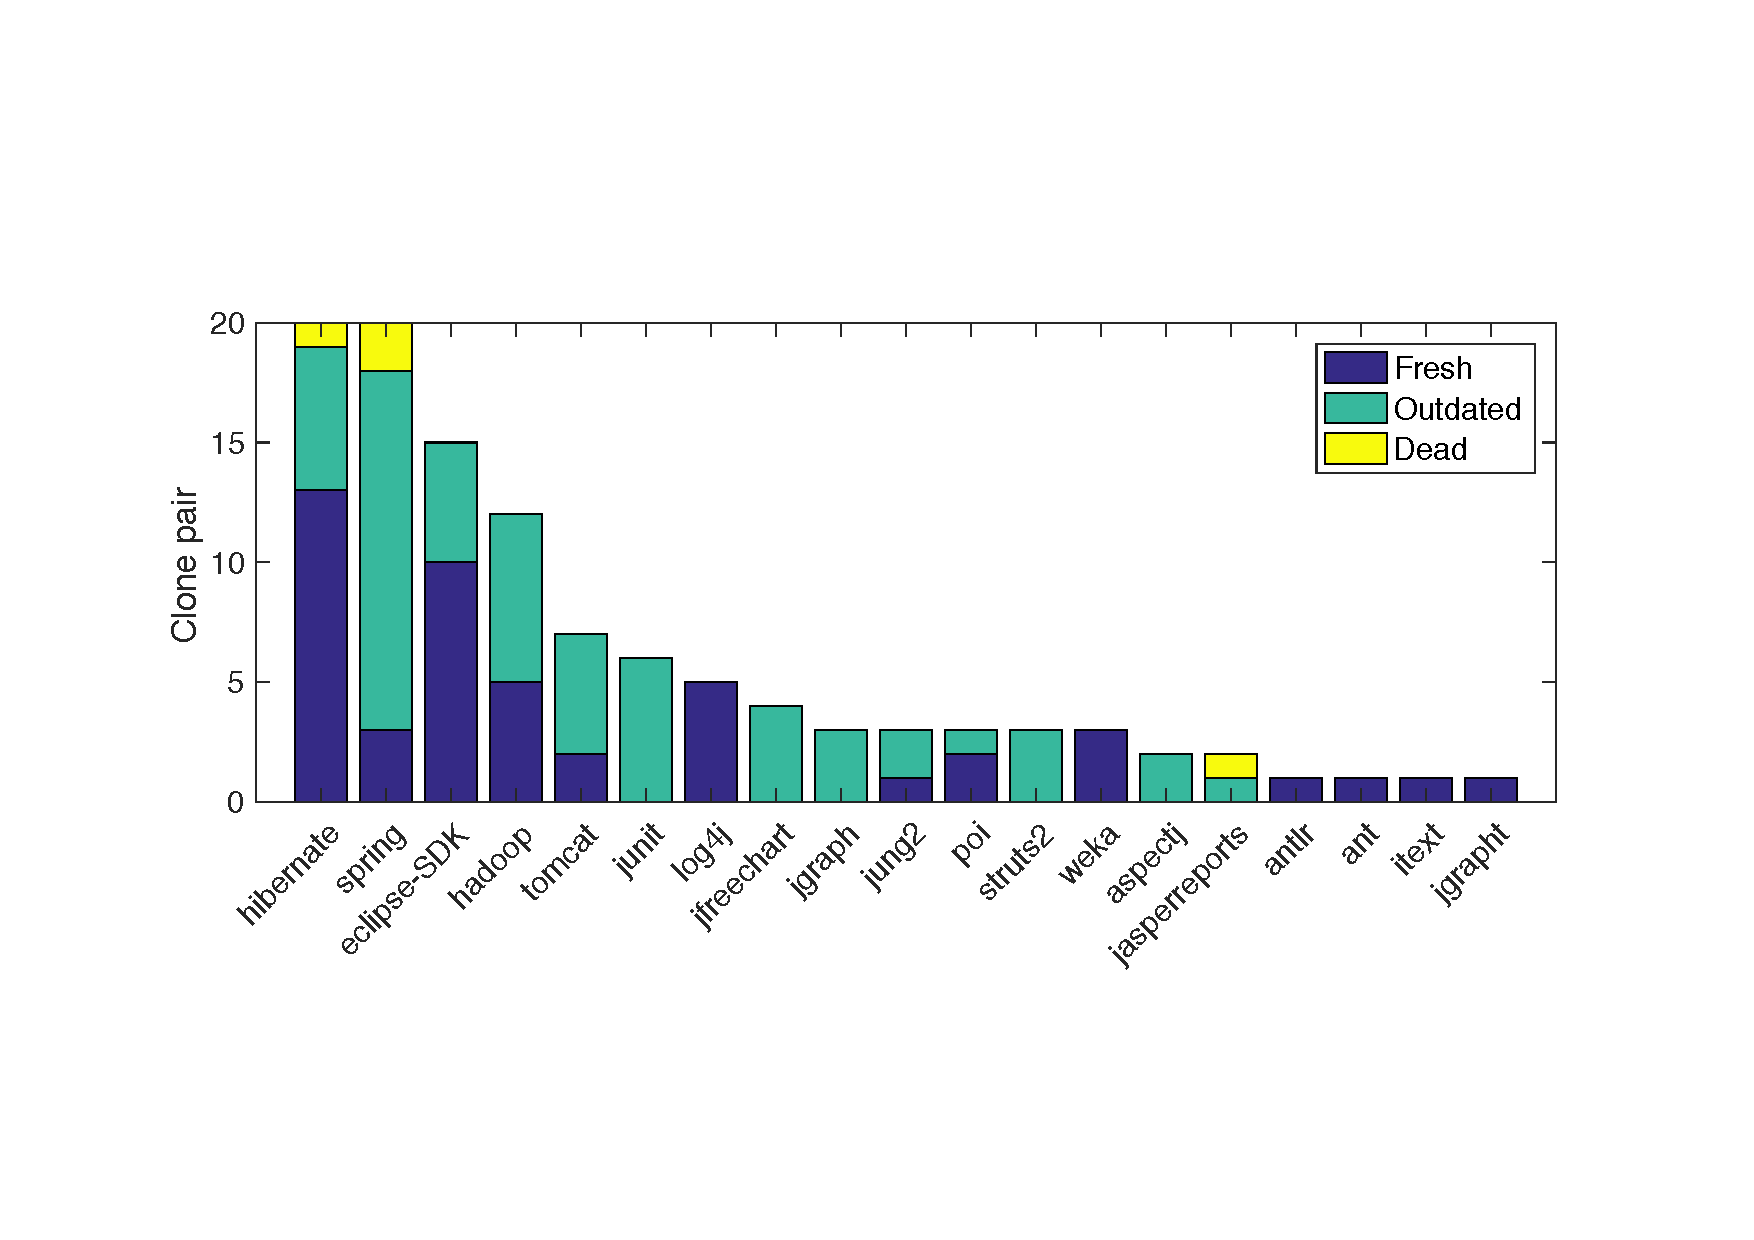
\includegraphics[width=\linewidth]{freshness}\vspace{-1ex}
	\caption{Status of the 112 QS online clone pairs}
	\label{fig:outdated}
\end{figure}

\begin{table*}
	\centering
	\caption{Examples of the outdated QS online clones}
	\label{tab:stale_code_details}
	\small
	%\resizebox{\textwidth}{!}{%
		\begin{tabular}{cc|lcp{5.15cm}@{}rrc|c@{}c}
		 \hline
		 \multicolumn{2}{c|}{Stack Overflow} & \multicolumn{6}{c|}{Qualitas} & \multicolumn{2}{c}{Changes} \\ 
		 \hline
		 Post & Date & Project & Ver. & File & Start & End & Date & Type$^*$ & Date \\
		 \hline
		 22315734 & 11-Mar-14 & hadoop & 1.0.0 & WritableComparator.java & 44 & 54 & 25-Aug-11 & \textit{S} & 20-Nov-14 \\
		 23520731 & 7-May-14 & hibernate & 4.2.2 & SchemaUpdate.java & 115 & 168 & 22-May-13 & \textit{S} & 5-Feb-16 \\
		 21734562 & 12-Feb-14 & tomcat & 7.0.2  & FormAuthenticator.java & 51 & 61 & 4-Aug-10 & \textit{R} & 4-Aug-16 \\
		 12593810 & 26-Sep-12 & poi & 3.6 & WorkbookFactory.java & 18 & 28 & 7-Dec-09 & \textit{R} & 26-Jun-13 \\
		 8037824 & 7-Nov-11 & jasperreports & 3.7.4 & JRVerifier.java & 1221 & 1240 & 31-May-10 & \textit{D} & 20-May-11 \\
		 3758110 & 21-Sep-10 & spring & 3.0.5  & DefaultAnnotationHandlerMapping.java & 78 & 92 & 20-Oct-10 & \textit{D} & 20-Jan-12 \\
		 \hline 
		 \multicolumn{10}{l}{{\footnotesize * \textit{S}:
                  modified/added/deleted statements, \textit{D}: file
                  has been deleted,  \textit{R}: method has been
                  rewritten completely}}
		\end{tabular} %
	%}
\end{table*}

\subsection{RQ4: Software Licensing Violation}



\begin{table}[]
	\centering
	\caption{License mapping of  online clones (file-level)}
	\label{tab:license_abc}
	\small
	%\resizebox{\columnwidth}{!}{%
	\begin{tabular}{l|p{1.95cm}l|rrr}
		\hline
		Type & Stack Overflow\newline (CC BY-NC-SA) & Qualitas & QS & EX & UD \\
		\hline
		Compatible & Apache2 & Apache2 &  0 & 0  & 1\\
		License	& EPLv1 & EPLv1 &  1 & 0 & 1\\
		& Sun (proprietary) & Sun (proprietary) & 0 & 1 & 0\\
		& MIT-like & MIT-like & 0 & 1 & 0\\
		& No license & CC BY-NC-SA & 0 & 5 & 0 \\
		& No license & No license & 5 & 4 & 21 \\
		\hline
		\multicolumn{3}{l|}{Total} & 6 & 11 & 23 \\
		\hline
	    Incompat. & BSD3 & GPLv2+ & 0 & 0 & 1 \\
		License	& No license & AGPLv3/3+ & 1 & 0 & 2 \\
		& No license & Apache-2 & 41 & 6 & 23 \\
		& No license & BSD3 & 3 & 4 & 28 \\
		& No license & CDDL or GPLv2 & 1 & 0 & 58 \\
		& No license & CDDLv1 & 0 & 1 & 0 \\
		& No license & EPLv1 & 7 & 0 & 10 \\
		& No license & GPLv2/2+/3+ & 2 & 62 & 32 \\
		& No license & LGPLv2/2.1+/3+ & 24 & 0 & 32 \\
		& No license & MPLv1.1 & 0 & 0 & 1 \\
		& No license & spdxBSD3 & 0 & 0 & 10 \\
		& No license & SPLv1 & 0 & 1 & 0 \\
		& No license & Unknown & 0 & 3 & 3 \\
		& spdxBSD3 & AGPLv3+ & 0 & 0 & 2 \\
		\hline
		\multicolumn{3}{l|}{Total} &  79 & 77 & 202 \\
		\hline
	\end{tabular} %
%}
\end{table}


%If developers copy and reuse these licensed pieces of code in their projects, conflicts may happen without their realisation.
In our study, we reveal another possible situation of software
licensing issues caused by code cloned to Stack Overflow. We found
evidence that 112 pieces of code have been copied from Qualitas
projects to Stack Overflow as examples. Their status of accepted
answers increase their chances of being reused. Even though most of
the Qualitas projects came with a software license, we found that the license information
were frequently missing after the code was copied to Stack
Overflow. The licensing terms on top of source code files are not
copied because usually only a small part of the file was
cloned. In overall, we can see that most of the Stack Overflow snippets do not
contain licensing terms while their clone counterparts in Qualitas
projects do. The summary of
licensing information is listed in \Cref{tab:license_abc}.

\textbf{Compatible license:} There are 40 pairs which have compatible
licenses such as \emph{Apache license v.2}; \emph{Eclipse Public
  License v.1 (EPLv1)}; or a pair of no license vs.~\emph{Creative
  Common Attribution-NonCommercial-ShareAlike 3.0 Unported (CC
  BY-NC-SA 3.0)}. These clones are safe for being reused. Since source
code and text on Stack Overflow are
protected by \emph{CC BY-NC-SA 3.0}
, we can treat the Stack Overflow code snippets
without licensing information as having \emph{CC BY-NC-SA 3.0} by
default. The \emph{CC BY-NC-SA 3.0} license is relaxed and it only
requests an attribution when reused.

\textbf{Incompatible license:} there are 358 clone pairs which do not
contain licensing information after they are posted on Stack Overflow
or contain a different license from their Qualitas clone
counterparts. More than half (79) of \textbf{QS} clone pairs have
their licensing terms removed or changed when posted on Stack
Overflow. For \textbf{EX} clone pairs, we searched for licensing terms of the
original source code from the external sources. We found that 77 out
of 88 EX clone pairs have incompatible licenses.
%They are clones that have been identified to be copied from an external source.
Similarly, the license statement was removed from Stack Overflow
snippets. Of 226 \textbf{UD} clone pairs, 202 pairs have incompatible
licenses. Again, most clones in Qualitas contain a license
while the Stack Overflow snippets do not.
%
%\Cref{fig:sankey_license} shows the direction of changes in online code clone license. The direction of the change is from left to right. The thickness of the line reflects the number of clones for that relationship. In \Cref{fig:sankey_license} (A), we can clearly see that most of the QS online clones have their licenses changed from having a license to ``No license'' on Stack Overflow. The same findings were found for EX online clones as depicted in \Cref{fig:sankey_license} (B). We found that most of the EX clones have their licensing information stripped of after copying to Stack Overflow. These clones are instead covered by the default CC BY-NC-SA 3.0 license of Stack Overflow which is strongly permissive. These used-to-be-licensed code are dangerous for being reused because they can implicitly conflict with the reused software's license.

\textbf{For RQ4, we found 358 code snippets on Stack Overflow that
  violate the license of their original software. The majority of them
  do not contain licensing statements after they have been copied to
  Stack Overflow.}

\section{Overall Discussion}
%What can we learn for the results? For example, if a developer explicitly reports in his/her code that the snippet was copied from stackoverfow, are there some benefits? We could notify - for instance - the developer when some new issues related to the snippet are posted on stackoverflow? Or could we force people posting code on SO to explicitly report licensing information? Or, could we implement an intelligent IDE that when pasting code from external resource checks for licensing violation? These of course are only some (crazy?) ideas that could be developed on the top of the results we have achieved with this study... 

%We discovered two issues regarding code snippets on Stack Overflow in this study: (1)  outdated online clones on Stack Overflow and (2) missing or incompatible license in Stack Overflow snippets. 
%that there is a considerable amount of cloned code between Stack Overflow that are cloned from 111 projects in the Qualitas corpus. 64 clone pairs are outdated and 358 snippets have incompatible software licenses to their originals. 
Our study discovers links from code in open source projects to code
snippets on Stack Overflow using clone detection techniques. These
links enable us to discover outdated code and licensing problems. The
links can be exploited further to mitigate the problems of reusing
outdated online clones and incompatible license on Stack Overflow code
snippets. We propose the following actionable items:

\textbf{Preventive measure:} We encourage Stack Overflow to enforce attribution when source code snippets have been copied ``from'' licensed software projects to Stack Overflow. Moreover, an IDE plug-in that can automatically detect pasted source code and follow the link to Stack Overflow and then to the original open source projects, could also prevent the issue of license violation.

\textbf{Detective measure:} A system to detect outdated source code
snippets on Stack Overflow is needed. The system can leverage the
online clone detection techniques in this study to periodically check
if the cloned snippets are still up-to-date with their
originals. %Moreover, Stack Overflow posters have to provide the information of the project including the original file name and its online repository (if exists).
With such a system, the poster can be notified when the code has been
updated in the original project so that he/she can update their code
on Stack Overflow accordingly. On the other hand, with a crowdsourcing
solution using an IDE plug-in, developers can also report the
corrected version of outdated code back to the original Stack Overflow
threads when they reuse outdated code and make corrections to them.

\section{Threats to Validity}

\textbf{Internal validity:} 
%
We could not verify all the 315,786,118 clone pairs reported by the
clone detection tools in this study.  Nevertheless, we applied
different mechanisms to ensure the validity to the subset of clone
pairs we classified.  First, we used two widely-used
clone detection tools, Simian and NiCad.  We tried three other
clone detectors but could not add them to the study due to their
scalability issues and susceptibility to incomplete code snippets.
Second, we adopted Bellon's agreement metric~\cite{Bellon2007}
to prioritise and filters clone pairs for the manual
classification. The agreed clone pairs that passed \textit{good}- and
\textit{ok}- criteria had a higher chance to be true positive. 
Nevertheless, we might still suffers from false negatives, i.e.~online 
code clones that are not reported by the tools or are filtered 
out by the automatic classifier before the manual investigation.
% We also
% applied the Bellon's clone agreement to 4 different combinations of
% the tools' configurations.  For disagreed clone pairs, we applied
% several filters to remove spurious and uninteresting clones.

% The number of online clones we found are subject to the clone
% detectors and their configurations.  
We mitigated the problem of clone
detector's parameter sensitivity by adding another established
configuration from the EvaClone study~\cite{Wang2013}. 

% We also
% performed a pairwise matching between the default and EvaClone
% configurations of the two clone detection tools.

Our seven patterns of online code cloning may not cover all possible
online cloning patterns. However, instead of defining the patterns
beforehand, we resorted to extract them from the data sets. We derived
them from a manual investigation of 679 online clone pairs and adopted
one pattern from the study by Kapser et al.~\cite{Kapser2003}.

The 3,636 clone pairs classified manually by the first author are
subject to manual judgement and human errors.  Although we have tried
our best to be careful on searching for evidence and classifying the
clones, some errors may still exist. We mitigated this problem by
having the second author to validate the classifications with a random
sampling. 
% The 64 classification conflicts were discussed and
% resolved.  
The third author made a final judgement when no consensus
could be found by the two authors. This validation process
can be even improved by employing an external investigator. 
 %In addition, we are aware of voting mechanism
%in Stack Overflow and plan to incorporate highest-vote answers in the future work.

\textbf{External validity:} We carefully chose the data sets for our
experiment so the findings could be generalise as much as possible.
We selected Stack Overflow because it is one of the most popular
programming Q\&A websites available with approximately 6.8 million
users.  There are a large number of code snippets reused from the
site~\cite{An2017} and there are also several studies encouraging of
doing
so~(e.g.~\cite{Ponzanelli2013,Ponzanelli2014,Keivanloo2014,Park2014}).
Nonetheless, it may not be representative to all the programming Q\&A
websites.

Regarding the code snippets, we downloaded a full data dump and
extracted Java accepted answers
% Instead of analysing every post, we
%only focused on posts marked as accepted answers 
since they are the
most likely ones to be reused. 
% This yields a total of 144,064 snippets.  
Our findings are limited to these restrictions. They may
not be generalised to all programming languages and all answers on
Stack Overflow. We chose the curated Qualitas
corpus for Java open source projects containing 111 projects
\cite{QualitasCorpus}.  The projects span over several areas of
software and has been used in several empirical
studies~\cite{Taube-Schock2011,Beckman2011,Vasilescu2011,Omar2012}. Although
it is a curated and well-established corpus, it may not fully
represent all Java open source software available.

%Lastly, two clone detection tools, Simian and NiCad, are chosen for this study. We have not tried all the tools available and they might not be complete representatives of all available clone detection tools.

\section{Related Work}

\textbf{Stack Overflow} is a gold mine for software engineering
research and
% Its rich and developer-driven data are invaluable. Since
% posts on Stack Overflow may contain code snippets embedded within
% natural language text, they become a huge database for source code and
% code-relevant information. 
%The Stack Overflow data set 
has been put to
use in several previous studies. In terms of developer-assisting
tools, Seahawk is an Eclipse plug-in that searches and recommends
relevant code snippets from Stack Overflow~\cite{Ponzanelli2013}. A
follow up work, Prompter, by Ponzanelli et al.~\cite{Ponzanelli2014}
achieves the same goal but with improved algorithms. The code snippets
on Stack Overflow are mostly examples or solutions to programming
problems. Hence, several code search systems use whole or partial data
from Stack Overflow as their code search
databases~\cite{Keivanloo2014,Park2014,
  Stolee2014,Subramanian2013,Diamantopoulos2015}. Furthermore, Treude
et al.~\cite{Treude2016}~use machine learning techniques to extract
insight sentences from Stack Overflow and use them to improve API
documentation.

Another research area is knowledge extraction from Stack
Overflow. Nasehi et al.~\cite{Nasehi2012}~studied what makes a good
code example by analysing answers from Stack Overflow. Similarly, Yang
et al.~\cite{Yang2016} report the number of reusable code snippets on
Stack Overflow across various programming languages. Wang et
al.~\cite{Wang2013_StackOverflow} use Latent Dirichlet Allocation
(LDA) topic modelling to analyse questions and answers from Stack
Overflow so that they can automatically categorise new
questions. There are also studies trying to understand developers'
behaviours on Stack Overflow,
e.g.~\cite{Movshovitz-Attias2013,Rosen2016,Choetkiertikul2015,Bosu2013}.
% , while some studies aim to improve Stack Overflow itself~\cite{Diamantopoulos2015, Wang2014}. 

\textbf{Code clone detection} is a long-standing research topic in
software engineering. Whether clones are good or bad for software is
still
controversial~\cite{Sajnani2016,Kapser2003,Kapser2008,Krinke2008,Hotta2010,Gode2011,Harder2013}.
% However, by only knowing how many code clones residing in software
% and how they evolve~\cite{Pate2013,Mondal2011} can provide several
% valuable insights into the software systems.
Code clones have several
applications such as software plagiarism
detection~\cite{Prechelt2002}, source code
provenance~\cite{Davies2013}, and software licensing
conflicts~\cite{German2009}.

Two code fragments are clones if they are similar enough according to
a given definition of similarity~\cite{Bellon2007}. Given an open
interpretation of ``definition of similarity'', there are various
clone detection tools and their siblings, code plagiarism detectors,
invented based on plethora of different code similarity
measurements~\cite{Roy2008, Ragkhitwetsagul2016,Svajlenko2014}. 
% Some tools use string comparison techniques such as Simian~\cite{simian}. 
% NiCad~\cite{Roy2008,Cordy} exploits the Longest Common Subsequence
% (LCS) string similarity measure after applying code pretty-printing
% using TXL~\cite{Cordy2006}. 
Many tools do not work on original source code directly but detect clones
at an intermediate representation such as tokens ~\cite{Sajnani2016,Kamiya2002,Li2006,Gode2009,Burrows2007, Smith2009, Duric2012, Prechelt2002, Schleimer2003}, AST~\cite{Baxter1998,Jiang2007a} or program dependence
graphs~\cite{Krinke2001,Komondoor2001}. 

\textbf{Cloning patterns} is initially defined 
by Kapser et al.~\cite{Kapser2003,Kapser2008} by studying clones in 
Linux file systems and deriving 11 patterns of code cloning. 
Our study adopted one of the patterns into our online code cloning patterns.

\textbf{Clone agreement} is useful when a clone oracle is
absent. %Since clone detectors are different in their detection
%approaches, they may behave differently and report different clones
%even on the same data set. 
By exploiting the different behaviours of clone detectors,
one can look for their agreement and obtain
highly-confident clones~\cite{Bellon2007,Wang2013}. %Using the same
%data set, 
Clone pairs that are agreed by multiple tools are more assured to be true
clones than the ones reported by only a single
tool~\cite{Wang2013,cr2016ssbse,Funaro2010}. 
% There are studies that report sensitivities of the tools'
% configurations to the results~\cite{Wang2013,cr2016ssbse}, showing
% that searching for an optimal configuration for every new data set
% is preferred.

\textbf{Software licensing} is crucial for open source and 
industrial software development. Di Penta et al.~\cite{DiPenta2010}
studied the evolution of software licensing in open source 
software and found that licensing statements change over 
time. German et al.~\cite{German2009} found that licensing 
conflicts occur between the clone siblings, i.e.~clones among 
different systems that come from the same source. Later, 
German et al.~\cite{German2010} created an automated tool 
for software license identification, Ninka, which is used
in our online clone license analysis. 
%We use Ninka to analyse software license from Stack 
%Overflow snippets and Qualitas projects. 

\textbf{Reusing of outdated third-party source code} occurs 
in software development. Xia et al.~\cite{Xia2014} show that 
a large number of open source systems reuse outdated third-party 
libraries from popular open source projects. Using the outdated 
code give detrimental effects to the software since they may 
introduce vulnerabilities. Our study discovers similar findings 
in the context of outdated code on Stack Overflow.

The work that is closely similar to us is a study by 
An et al.~\cite{An2017} where the authors investigated 
clones between 399 Android apps and Stack Overflow posts. 
They found 1,226 code snippets which were reused from 68 Android apps. 
They also observed that there are 1,219 cases of potential 
license violations. The authors rely on the timestamp to 
judge whether the code has been copied from/to Stack Overflow 
along with confirmations from six developers. Instead of Android apps, 
we investigated clones between Stack Overflow and 111 open 
source projects. Their results are similar to our findings that 
there exist clones from software projects to Stack Overflow with 
potential licensing violations. 
%In our work, we defined seven patterns of online code cloning and 
%performed a large-scale manual check of 3,632 clone pairs. 
%We discovered 112 clone pairs with strong evidences, 
%based on natural text in comments and post contents, that they 
%were copied from Qualitas to Stack Overflow. By comparing the 
%clones to their latest versions in the software, we found that 
%64 code snippets on Stack Overflow are outdated and possibly harmful for reuse.

%\section{Future Work}
%Since this study is limited to only Java language, we are interested in expanding the study further to other popular programming languages such as C, C++, Python, and Javascript on Stack Overflow. The similar study of outdated code and software licensing violation can be repeated. It is interesting to compare the findings among different programming languages. Moreover, other popular software project corpora (e.g.~GitHub) can also be included to increase generalisation of the findings.
%
%We are eager to tackle the issues of outdated and license-violating online code clones with an automated tool. The tool should incorporate a scalable clone detection method of locate similar code from programming Q\&A websites such as Stack Overflow and online code repositories like GitHub. It analyses a software project under development and reports clones that are copied from Stack Overflow. The reported clones have traces to their origins in open source projects or websites along with their freshness (fresh/outdated/dead) so that the developer of the project can be aware of changes made to the copied code snippets. Lastly, the license of the original source code is also reported so the developer can make an informed decision of whether he or she will incorporate that code snippet into their own project.

\section{Conclusions}

Online code clones are clones that have been copied to Q\&A websites
such as Stack Overflow. 
% They are similar to classical clones in software
% projects where they can be outdated and violating software license but
% are much harder to detect. 
We classified 32,533 clone pairs using seven patterns of online code
cloning.  After automatically removing boiler-plate clones, we
manually investigated 3,636 clone pairs. In the 1,216 manually
confirmed clone pairs, we discovered 112 clone pairs that have been
copied, with evidence, from Qualitas projects to Stack Overflow, 197
clone pairs that have been copied from external sources besides
Qualitas to Stack Overflow, and 359 clone pairs that are highly
similar but without evidence of copying.

We performed a detailed analysis of the online clone pairs on two
aspects: outdated code and licensing violation. The investigation of
the 112 clone pairs copied, with evidence, from Qualitas to Stack
Overflow reveals that 64 of them are outdated.  Moreover, we found 358
code snippets on Stack Overflow that violate the license of their
original software.

This study is among, if not the first, to address the important issues
of outdated and license-violating online code clones on programming
Q\&A websites using a hybrid methodology of automatic code clone
detection and a manual clone investigation.

%
% The following two commands are all you need in the
% initial runs of your .tex file to
% produce the bibliography for the citations in your paper.
\bibliographystyle{ACM-Reference-Format}
\bibliography{sigproc}  

% \begin{table}
% 	\centering
% 	\caption{Statistics of online clones reported by Simian (\textit{S}) and NiCad (\textit{N}) with default (\textit{D}) and EvaClone (\textit{E}) configurations}
% 	\label{tab:raw_stats}
% 	%\small
% 	%\resizebox{\columnwidth}{!}{%
% 		\begin{tabular}{l|r|r|r|r}
% 			\hline
% 			Stats & \multicolumn{1}{c|}{$S_D$} & \multicolumn{1}{c|}{$S_E$} & \multicolumn{1}{c|}{$N_D$} & \multicolumn{1}{c}{$N_E$} \\
% 			\hline
% 			Stack Overflow Snippets & 1,086 & 1,531 & 1,392 & 12,886 \\
% 			No. of Qualitas projects & 92 & 111 & 82 & 88 \\
% %			Total C$_{\textrm{\textit{pairs}}}$ & 67,570 & 63,635,844 & 632,855 & 251,449,849 \\
% %			Avg.~C$_{\textrm{\textit{pairs}}}$ & 62 & 41,565 & 455 & 19,356 \\
% %			Avg.~C$_{\textrm{\textit{size}}}$ & 9.11 & 5.95 & 10.85 & 6.28 \\
% 			Avg.~C$_{\textrm{\textit{\%}}}$ & 38\% & 50\% & 30\% & 33\% \\
% 			\hline
% 		\end{tabular} %
% 	%}
% \end{table}

% \begin{figure*}
% 		\centering
% 		\begin{minipage}{.4\textwidth}
% 			\centering
% 			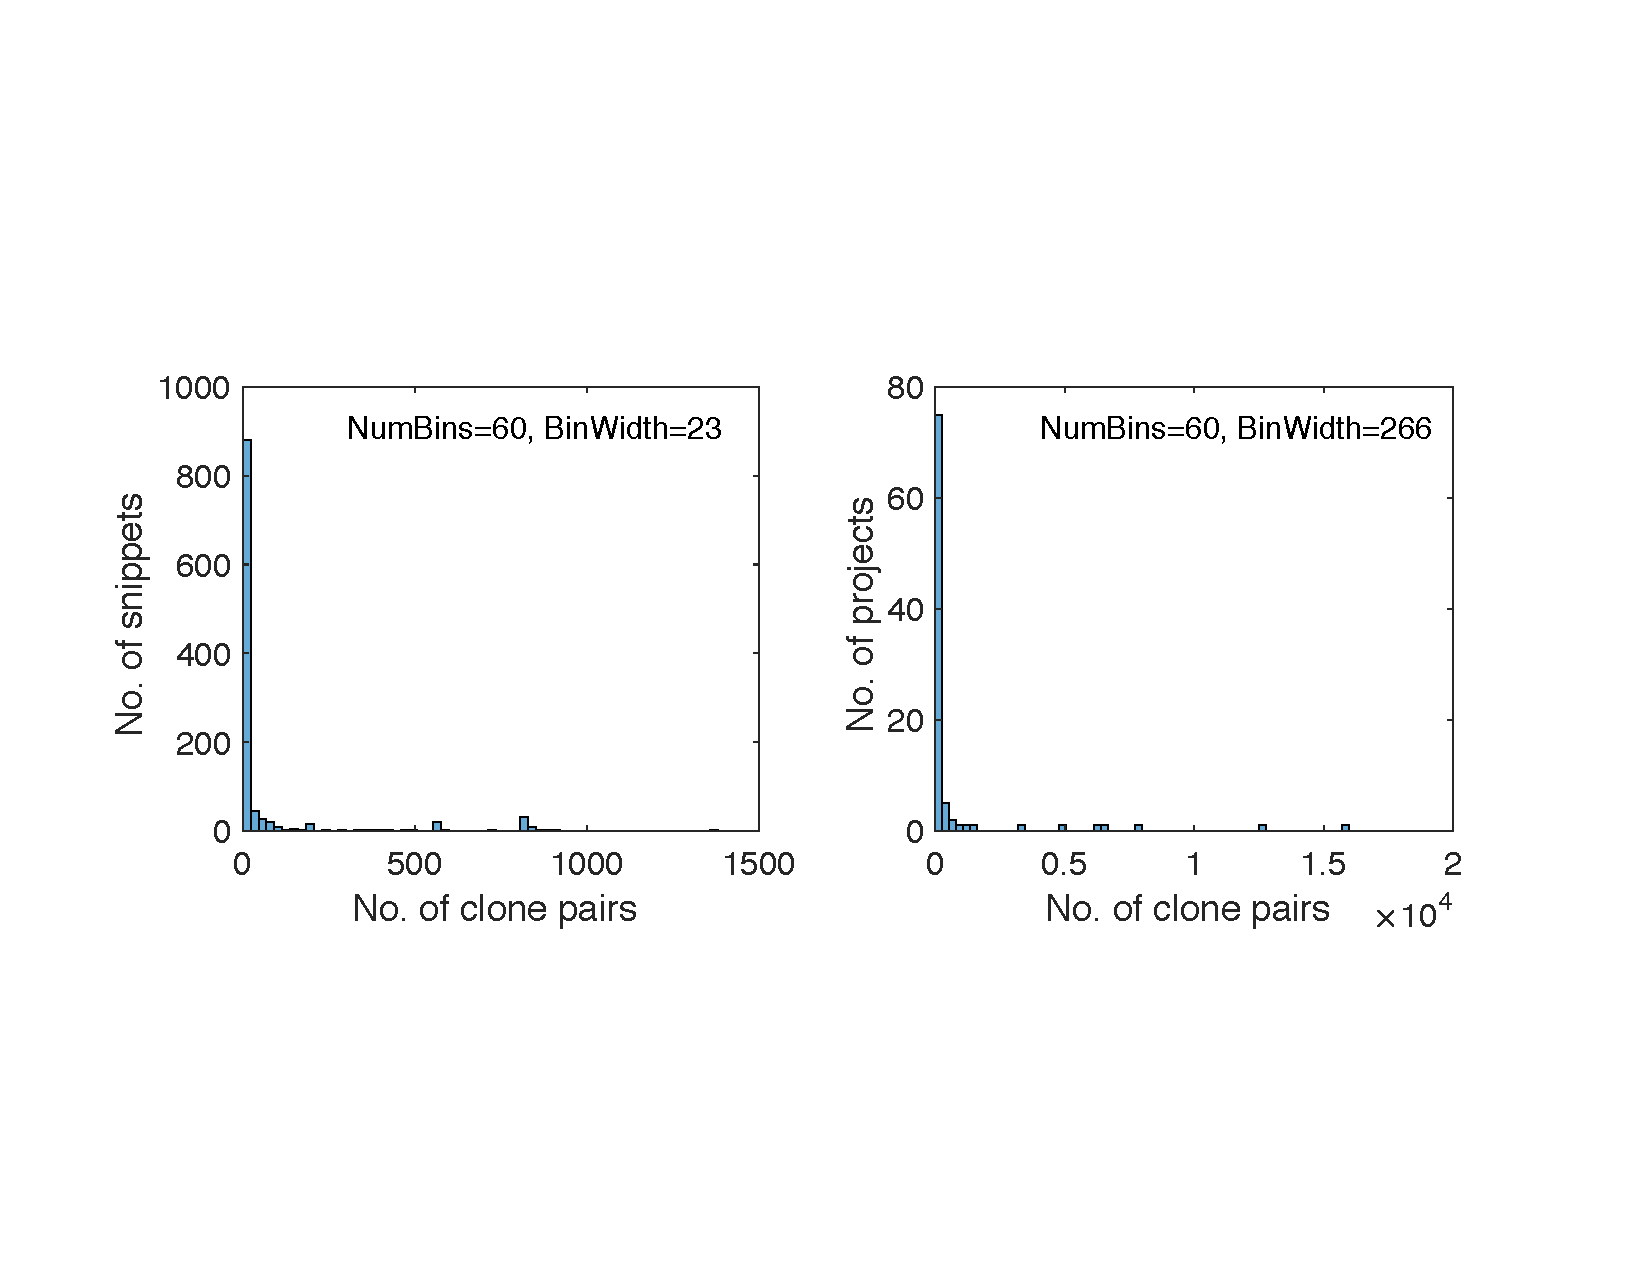
\includegraphics[width=\linewidth]{hist_sd}
% 			\caption*{$S_D$ clones}
% 		\end{minipage}%
% 		\hspace{5ex}
% 		\begin{minipage}{0.4\textwidth}
% 			\centering
% 			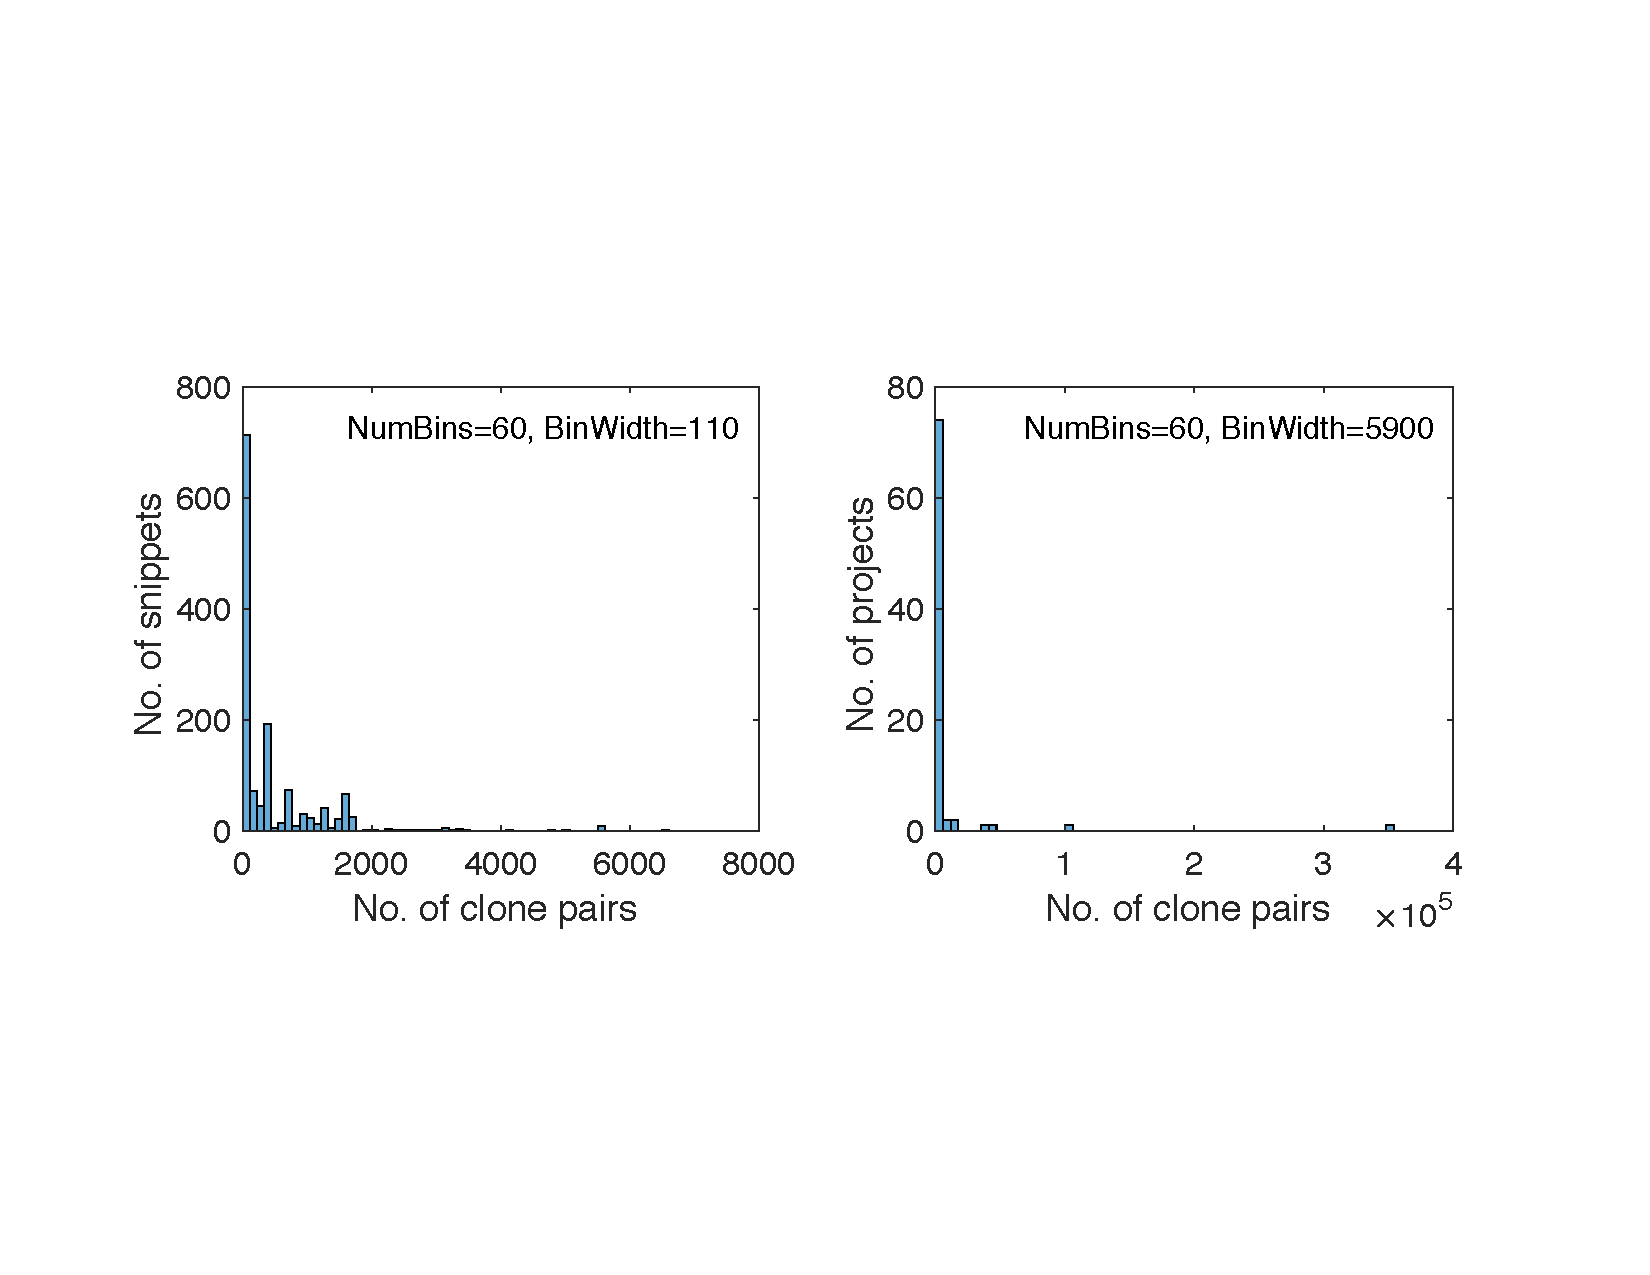
\includegraphics[width=\linewidth]{hist_nd}
% 			\caption*{$N_D$ clones}
% 		\end{minipage}
% 		\\
% 		\begin{minipage}{.4\textwidth}
% 			\centering
% 			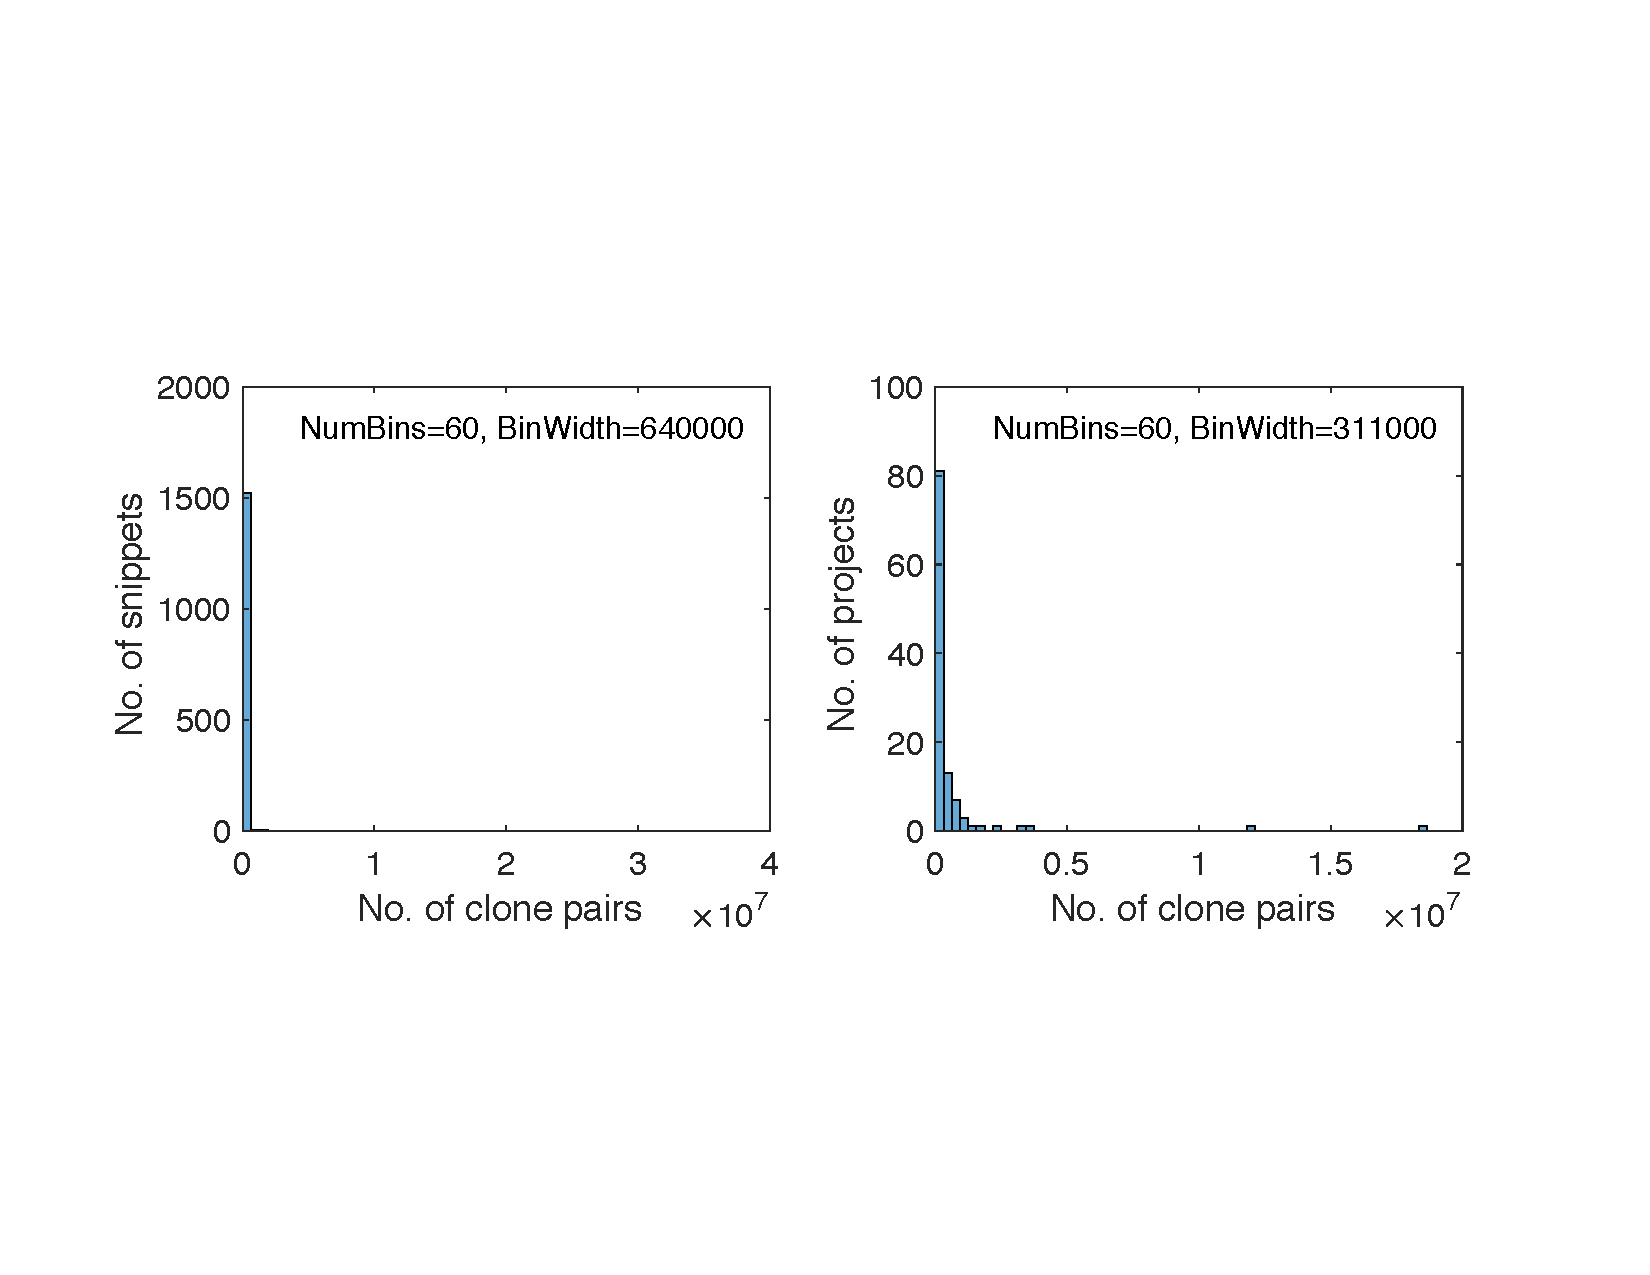
\includegraphics[width=\linewidth]{hist_se}
% 			\caption*{$S_E$ clones}
% 		\end{minipage}%
% 		\hspace{5ex}
% 		\begin{minipage}{0.4\textwidth}
% 			\centering
% 			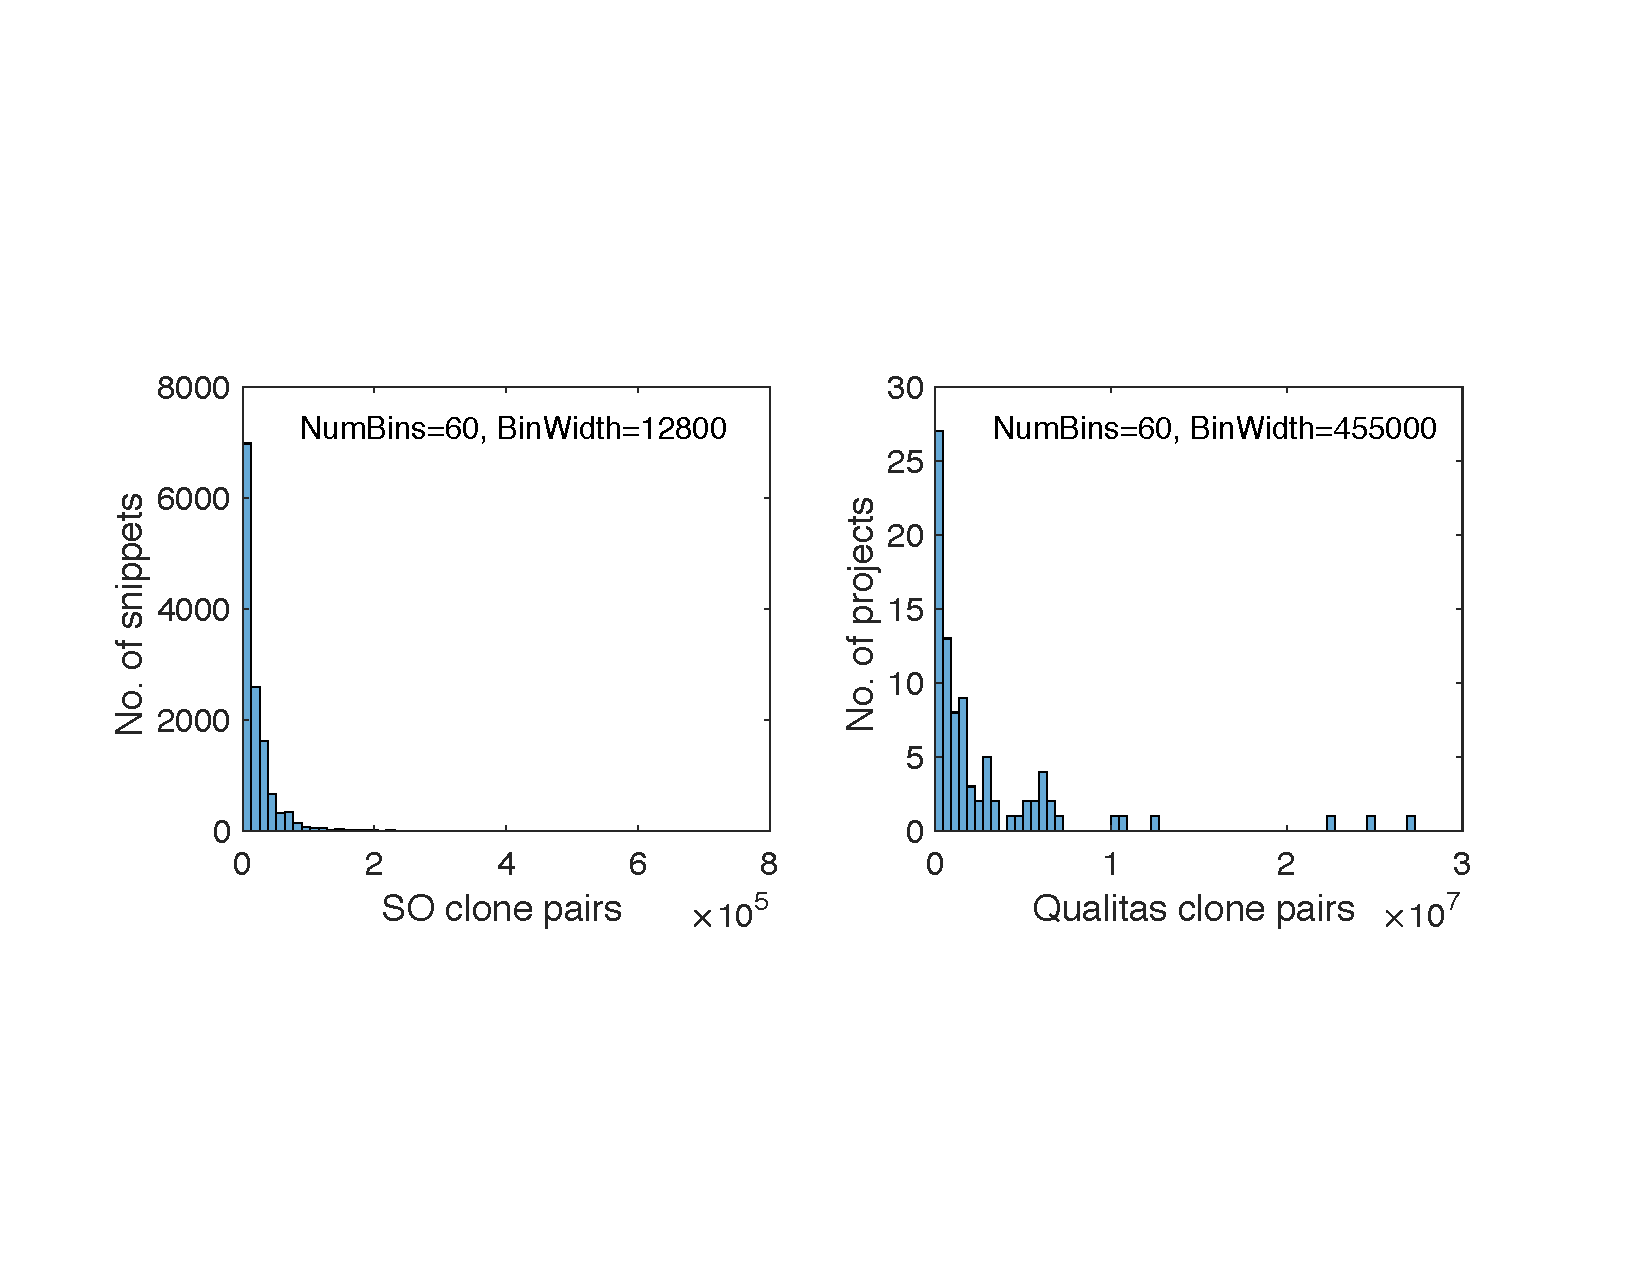
\includegraphics[width=\linewidth]{hist_ne}
% 			\caption*{$N_E$ clones}
% 		\end{minipage}
% 	\caption{\FIXME{Useful?}~Distribution of online clones between Stack Overflow snippets and Qualitas projects}
% 	\label{fig:histogram}
% \end{figure*}

%They do not exist any more in the latest version.} %These outdated Stack Overflow online clone snippets are questionable for reuse.} %These changes did not reflect They might later find out that the copied code does not work any more due to different API versions. Even worse, they might also introduce bugs or vulnerabilities into their software.  }
%Usually when developers reuse a code snippet from a Stack Overflow post and find that it does not work nor compatible with their environment. They can cast a down vote to that answer resulting in low votes for the answer (which might be outdated). However, if the answer is marked as accepted by the person who asks the question, the check mark symbol attached to the answer is still attractive to naive developers who are ignorant. 

%\begin{figure*}
%	\begin{lstlisting}
%          /* Code in Stack Overflow #23520731 */             /* SchemaUpdate.java (2016-09-26) */
%          public void execute (Target target) {              public void execute(EnumSet<TargetType> targetTypes, 
%            LOG.runningHbm2ddlSchemaUpdate();                                Metadata metadata, ServiceRegistry serviceRegistry) {
%            Connection connection = null;                      if ( targetTypes.isEmpty() ) {
%            Statement stmt = null;                               LOG.debug(""Skipping SchemaExport as no targets were specified"");
%            Writer outputFileWriter = null;                      return;
%            exceptions.clear();                                }
%            try {                                              exceptions.clear();
%              DatabaseMetadata meta;                           LOG.runningHbm2ddlSchemaUpdate();
%              ...                                              ...
%	\end{lstlisting}
%	\caption{Outdated code snippet on Stack Overflow post 23520731. This code has been copied from {\small\texttt{SchemaUpdate.java}}. Its latest version in \textsf{hibernate} code base contains heavy modifications.}
%	\label{fig:hibernate_outdated_code}
%\end{figure*}

%\begin{table*}
%	\centering
%	\caption{Examples of the 6 outdated QS online clones. Outdated clones are caused by modified/added/deleted statements (\textit{S}), file deletion (\textit{D}), and method rewriting (\textit{R}).}
%	\label{tab:stale_code_details}
%	\small
%	\resizebox{2\columnwidth}{!}{%
%	\begin{tabular}{r|l|l|l|l|p{5.2cm}|r|r|l|c|l}
%		\hline 
%		\multirow{2}{*}{No.} & \multicolumn{2}{c|}{Stack Overflow} & \multicolumn{6}{c|}{Qualitas} & \multicolumn{2}{c}{Changes} \\ \cline{2-11}
%		& Post & Date & Project & Ver. & File & Start & End & Date & Type & Date \\
%		\hline
%			1 & 18303692 & 18-Aug-13 & aspectj & 1.6.9  & aspectjtools/../Agent.java & 7 & 18 & 5-Mar-08 & \textit{S} & 8-Sep-15 \\
%			2 & 18303692 & 18-Aug-13 & aspectj & 1.6.9  & aspectjweaver/../Agent.java & 7 & 18 & 5-Mar-08 & \textit{S} & 8-Sep-15 \\
%			3 & 2513183 & 25-Mar-10 & eclipse-SDK & 4.3 & GenerateToStringAction.java & 113 & 166 & 5-Jun-13 & \textit{S} & 17-Mar-15 \\
%			4 & 2513183	& 25-Mar-10 & eclipse-SDK & 4.3 & GenerateToStringAction.java & 117 & 126 & 5-Jun-13 & \textit{S} & 17-Mar-15 \\
%			5 & 2513183	& 25-Mar-10 & eclipse-SDK & 4.3 & GenerateToStringAction.java & 143 & 165 & 5-Jun-13 & \textit{S} & 1-Mar-11 \\
%			6 & 2513183	& 25-Mar-10 & eclipse-SDK & 4.3 & GenerateToStringAction.java & 178 & 187 & 5-Jun-13 & \textit{S} & 5-Jun-13 \\
%			7 & 11861598 & 8-Aug-12 & eclipse-SDK & 4.3 & WizardDialog.java & 377 & 394 & 1-May-13 & \textit{S} & 21-Jun-13 \\
%			8 & 22315734 & 11-Mar-14 & hadoop & 1.0.0 & WritableComparator.java & 44 & 54 & 25-Aug-11 & \textit{S} & 20-Nov-14 \\
%			9 & 801987 & 29-Apr-09 & hadoop & 1.0.0 & StringUtils.java & 40 & 56 & 15-Dec-11 & \textit{S} & 4-Feb-13 \\
%			10 & 21702608 & 11-Feb-14 & hadoop & 1.0.0 & DBCountPageView.java & 275 & 287 & 15-Dec-11 & \textit{S} & 12-Jun-11 \\
%			11 & 21702608 & 11-Feb-14 & hadoop & 1.0.0 & DBCountPageView.java & 289 & 309 & 15-Dec-11 & \textit{S} & 12-Jun-11 \\
%			12 & 14845581 & 13-Feb-13 & hadoop & 1.0.0 & JobSubmissionFiles.java & 46 & 55 & 15-Dec-11 & \textit{S} & 25-Jun-12 \\
%			13 & 16180910 & 24-Apr-13 & hadoop & 1.0.0 & mapred/../LineRecordReader.java & 47 & 60 & 15-Dec-11 & \textit{R} & 25-Jul-11 \\
%			14 & 16180910 & 24-Apr-13 & hadoop & 1.0.0 & mapreduce/../LineRecordReader.java & 41 & 54 & 15-Dec-11 & \textit{R} & 25-Jul-11 \\
%			15 & 15168494 & 24-Feb-14 & hibernate & 4.2.2 & ConnectionProviderInitiator.java & 65 & 93 & 22-May-13 & \textit{S} & 26-Apr-13 \\
%			16 & 24924255 & 24-Jul-14 & hibernate & 4.2.2 & Example.java & 224 & 243 & 22-May-13 & \textit{S} & 23-Apr-13 \\
%			17 & 23520731 & 7-May-14 & hibernate & 4.2.2 & SchemaUpdate.java & 115 & 168 & 22-May-13 & \textit{S} & 5-Feb-16 \\
%			18 & 8257554 & 26-Nov-11 & hibernate & 4.2.2 & SettingsFactory.java & 244 & 255 & 22-May-13 & \textit{D} & 11-Mar-11 \\
%			19 & 23967852 & 31-Apr-14 & hibernate & 4.2.2 & SQLServer2005LimitHandler.java & 43 & 61 & 22-May-13 & \textit{S} & 11-May-16 \\
%			20 & 19298607 & 10-Oct-13 & hibernate & 4.2.2 & Oracle9iDialect.java & 23 & 32 & 22-May-13 & \textit{S} & 12-Apr-15 \\
%			21 & 10031897 & 5-Apr-12 & hibernate & 4.2.2 & AliasToBeanResultTransformer.java & 44 & 61 & 22-May-13 & \textit{S} & 4-Jun-15 \\ 
%			22 & 8037824 & 7-Nov-11 & jasperreports & 3.7.4 & JRVerifier.java & 982 & 998 & 31-May-10 & \textit{S} & 17-Apr-08 \\
%			23 & 8037824 & 7-Nov-11 & jasperreports & 3.7.4 & JRVerifier.java & 1221 & 1240 & 31-May-10 & \textit{D} & 20-May-11 \\
%			24 & 12936580 & 17-Oct-12 & jfreechart & 1.0.13 & AbstractXYItemRenderer.java & 532 & 569 & 20-Apr-09 & \textit{S} & 16-Jan-16 \\
%			25 & 16058183 & 17-Apr-13 & jfreechart & 1.0.13 & KeyToGroupMap.java & 18 & 30 & 20-Apr-09 & \textit{S} & 29-Jun-07 \\
%			26 & 21998949 & 24-Feb-14 & jfreechart & 1.0.13 & SpiderWebPlot.java & 502 & 520 & 20-Apr-09 & \textit{S} & 2-Jun-08 \\
%			27 & 21998949 & 24-Feb-14 & jfreechart & 1.0.13 & SpiderWebPlot.java & 522 & 536 & 20-Apr-09 & \textit{S} & 22-Nov-13 \\
%			28 & 6722760 & 17-Jul-11 & jgraph & 5.13.0.0 & HelloWorld.java (3 overlaps)  & 14 & 37 & 25-Sep-09 & \textit{R} & 13-Apr-14 \\
%			31 & 6025026 & 17-Jul-11 & jung2 & 2\_0\_1  & ShortestPathDemo.java & 106 & 117 & 20-Jun-08 & \textit{S} & 13-Apr-10 \\
%			32 & 6025026 & 17-Jul-11 & jung2 & 2\_0\_1  & ShortestPathDemo.java & 158 & 172 & 20-Jun-08 & \textit{S} & 29-Nov-15 \\
%			33 & 23586872 & 31-May-14 & junit & 4.11 & Assert.java & 33 & 52 & 11-Oct-12 & \textit{S} & 12-May-15 \\
%			34 & 7504040 & 29-Sep-11 & junit & 4.11 & ExternalResource.java (3 overlaps) & 4 & 23 & 11-Oct-12 & \textit{S} & 25-Jun-16 \\
%			37 & 8802082 & 10-Jan-12 & junit & 4.11 & ExpectException.java (2 overlaps) & 11 & 29 & 11-Oct-12 & \textit{S} & 25-May-14 \\
%			39 & 12593810 & 26-Sep-12 & poi & 3.6 & WorkbookFactory.java & 18 & 28 & 7-Dec-09 & \textit{R} & 26-Jun-13 \\
%			40 & 20913543 & 6-Jan-14 & spring & 3.0.5  & AutowireUtils.java & 32 & 42 & 20-Oct-10 & \textit{S} & 28-Oct-14 \\
%			41 & 18623736 & 4-Sep-13 & spring & 3.0.5  & CustomCollectionEditor.java & 33 & 71 & 20-Oct-10 & \textit{S} & 21-Nov-13 \\
%			42 & 22865824 & 4-Apr-14 & spring & 3.0.5  & JavaMailSenderImpl.java & 169 & 185 & 20-Oct-10 & \textit{S} & 6-Oct-14 \\
%			43 & 22865824 & 4-Apr-14 & spring & 3.0.5  & JavaMailSenderImpl.java & 186 & 197 & 20-Oct-10 & \textit{S} & 6-Oct-14 \\
%			44 & 20421869 & 6-Dec-13 & spring & 3.0.5  & ClassPathScanningCandidateComponent\newline Provider.java (2 overlaps) & 85 & 133 & 20-Oct-10 & \textit{R} & 12-Aug-16 \\
%			46 & 3751463 & 20-Sep-10 & spring & 3.0.5  & ScheduledTasksBeanDefinitionParser.java & 42 & 52 & 20-Oct-10 & \textit{S} & 21-May-12 \\
%			47 & 6149818 & 27-May-11 & spring & 3.0.5  & DefaultPropertiesPersister.java & 69 & 80 & 20-Oct-10 & \textit{S} & 19-Mar-13 \\
%			48 & 10952561 & 8-Jun-12 & spring & 3.0.5  & HibernateTemplate.java & 761 & 769 & 20-Oct-10 & \textit{S} & 9-May-15 \\
%			49 & 10952561 & 8-Jun-12 & spring & 3.0.5  & Jaxb2Marshaller.java & 253 & 269 & 20-Oct-10 & \textit{S} & 28-Aug-12 \\
%			50 & 20996373 & 8-Jan-14 & spring & 3.0.5  & test/../DelegatingServletInputStream.java & 6 & 20 & 20-Oct-10 & \textit{S} & 18-Dec-08 \\
%			51 & 20996373 & 8-Jan-14 & spring & 3.0.5  & web/../DelegatingServletInputStream.java & 6 & 20 & 20-Oct-10 & \textit{S} & 15-Jul-16 \\
%			52 & 20996373 & 8-Jan-14 & spring & 3.0.5  & servlet/../ DelegatingServletInputStream.java & 6 & 20 & 20-Oct-10 & \textit{S} & 15-Jul-16 \\
%			53 & 5660519 & 15-Apr-11 & spring & 3.0.5 & AnnotationMethodHandlerException\newline Resolver.java & 224 & 233 & 20-Oct-10 & \textit{D} & 20-Jan-12 \\
%			54 & 4781746 & 24-Jan-11 & spring & 3.0.5  & DispatcherServlet.java & 91 & 103 & 20-Oct-10 & \textit{S} & 8-Aug-11 \\
%			55 & 3758110 & 21-Sep-10 & spring & 3.0.5  & DefaultAnnotationHandlerMapping.java & 78 & 92 & 20-Oct-10 & \textit{D} & 20-Jan-12 \\
%			56 & 9003314 & 25-Jan-12 & spring & 3.0.5  & WebDataBinder.java & 95 & 108 & 20-Oct-10 & \textit{S} & 15-Aug-10 \\
%			57 & 14019840 & 24-Dec-12 & struts2 & 2.2.1  & DefaultActionMapper.java & 128 & 144 & 17-Jul-10 & \textit{S} & 18-Oct-13 \\
%			58 & 15131432 & 28-Feb-13 & struts2 & 2.2.1  & FreemarkerManager.java & 163 & 177 & 17-Jul-10 & \textit{S} & 28-Oct-13 \\
%			59 & 15110171 & 27-Feb-13 & struts2 & 2.2.1  & StringLengthFieldValidator.java & 25 & 42 & 17-Jul-10 & \textit{S} & 15-Jun-15 \\
%			60 & 21734562 & 12-Feb-14 & tomcat & 7.0.2  & BasicAuthenticator.java (2 overlaps) & 25 & 73 & 4-Aug-10 & \textit{R} & 4-Aug-16 \\
%			62 & 21734562 & 12-Feb-14 & tomcat & 7.0.2  & FormAuthenticator.java & 51 & 61 & 4-Aug-10 & \textit{R} & 4-Aug-16 \\
%			63 & 24404964 & 25-Jun-14 & tomcat & 7.0.2  & CoyoteAdapter.java & 543 & 553 & 4-Aug-10 & \textit{S} & 25-Sep-14 \\
%			64 & 10289462 & 23-Apr-12 & tomcat & 7.0.2  & JspRuntimeLibrary.java & 252 & 296 & 4-Aug-10 & \textit{S} & 12-Sep-12 \\
%			\hline
%	\end{tabular} %
%}
%\end{table*}

\end{document}
